\documentclass[12pt]{report}
\usepackage[utf8]{inputenc}
\usepackage{graphicx}
\usepackage{hyperref}
\usepackage{wrapfig}
\hypersetup{pdftex,colorlinks=true,allcolors=black}
\usepackage{hypcap}
\graphicspath{ {images/} }
\usepackage{amsfonts}
\usepackage{amsmath}
\usepackage{amssymb}
\usepackage{subfig}
\usepackage{epsfig}
\usepackage{color}
\usepackage{geometry}
\usepackage{wrapfig}
\usepackage{eurosym}
\usepackage{titlesec, blindtext}
\usepackage[numbers]{natbib}
\usepackage{epigraph}
\usepackage{wrapfig}
\pagenumbering{Roman}


\begin{document}
	\begin{center}
		
		\Large \textbf{Optical Properties of Gain incorporating Photonic Resonators}
		
	\end{center}
\begin{center}
	\begin{figure}[h]
	\centering
	\includegraphics[width=5cm,height=7cm,keepaspectratio]{universitye.jpg}\\
	\end{figure}
\end{center}
	\begin{center}
		\emph{\large by}\\
		
		\Large \textbf{AHMAD BILAL}\\
		\Large CIIT/FA15-BPH-019/ISB\\
		\vfill
		\Large BS Thesis\\
		\Large In\\
		\Large Physics
	\end{center}
	\vfill
	\begin{center}
		\Large \textbf{COMSATS University Islamabad}\\
		\Large Islamabad - Pakistan
	\end{center}
	
	\begin{center}
		 January, 2019
	\end{center}
	\newpage
	\noindent
	\begin{wrapfigure}{l}{0.12\textwidth}
		\centering
		\includegraphics[width=0.8\linewidth]{university.jpg}
	\end{wrapfigure}
	\begin{center}
	{\Large{ \textbf{COMSATS University Islamabad}}}
	\end{center}
	
	\vspace{0.2 in}
	
	\begin{center}
		{\Large {Optical Properties of Gain incorporating Photonic Resonators
		} }
	\end{center}
	\vspace{0.5 in}
	
	\begin{center}
	{A Thesis Presented to}
	\end{center}
	\vspace{0.2 in}
	\begin{center}
		{\Large {\textbf{COMSATS University Islamabad}} }
	\end{center}
	\vspace{0.5 in}
	\begin{center}
		{In partial fulfillment }
	\end{center}

	\begin{center}
		{of the requirement for the degree of}
	\end{center}
	
	\vspace{0.5 in}
	
	\begin{center}
		{\Large {\textbf{Bachelor of Science in Physics}} }
	\end{center}
	
	\vspace{0.5 in}
	\begin{center}
		{by }
	\end{center}
	\begin{center}
		{\large {Ahmad Bilal\\[0pt]
				CUI/FA15-BPH-019/ISB\\[0pt]
		}}
	\end{center}
	\vspace{0.5 in}
	\begin{center}
		Spring, 2019
	\end{center}
	\newpage
	\begin{center}
{\Large {Optical Properties of Gain incorporating Photonic Resonators}\\[0pt]
		\noindent\rule{18cm}{3pt}} \\
\end{center}
\vspace{0.2 in} 
		A Under Graduate Thesis submitted to the Department of Physics as partial fulfillment of the requirement for the award of Degree of BS (Physics). 
\vspace{0.5 in}
\begin{center}
	\begin{tabular}{ | c| c | }
			\hline
			Name &  Registration Number \\
			\hline
		Ahmad Bilal & CUI/FA15-BPH-019/ISB \\ 
			\hline
	\end{tabular}
\end{center}
	\vspace{3 in}
	\textbf {Supervisor:}\\
	Dr. Ahmer Naweed,\\
	Associate Professor,\\
	Department of Physics,\\
	COMSATS University Islamabad (CUI),\\
	January, 2019.
	\newpage
	
	\begin{center}
		\textbf{\Large{Final Approval}}
		\noindent\rule{15cm}{1pt} \\

		This thesis titled\\
		\vspace{0.5cm}
{\Large \textbf {Optical Properties of Gain incorporating Photonic Resonators}}\\
\vspace{0.3cm}
By\\ar
\emph{Ahmad Bilal}\\
\emph{CIIT/FA15-BPH-019/ISB}\\
\vspace{0.1 in}
Has been approved\\
\vspace{0.1 in}
For the COMSATS University Islamabad\\
\end{center}
\vspace{0.5cm}
External Examiner: \noindent\rule{8cm}{0.4pt}\\\\\\\\\\\\
Supervisor: \hspace{1.35cm}\noindent\rule{8cm}{0.4pt}\\
\begin{center}
	Dr. Ahmer Naweed\\
	Associate Professor, Dept. of Physics\\
	COMSATS University Islamabad\\
\end{center}
\vspace{0.5cm}
HoD: \hspace{2.5cm}\noindent\rule{8cm}{0.4pt}\\
\begin{center}
	Dr. Sajid Qamar\\
	Professor, Dept. of Physics\\
	COMSATS University Islamabad
\end{center}
	\newpage
	\begin{center}
		\textbf{\Large{Declaration}}
		\end{center}
I \underline{\textbf{Ahmad Bilal} (CIIT/FA15-BPH-019/ISB)} hereby declare that this project
neither as a whole nor as a part there of has been copied out from any source. It is
further declared that I have developed this thesis and the accompanied report entirely
on the basis of my personal efforts made under the sincere guidance of my supervisors.
No portion of the work presented in this report has been submitted in support of any
other degree of qualification of this or any other University or Institute of learning, if
found I shall stand responsible.  \\\\\\\\\\
Date: \underline{}  \\\\\\
\begin{flushright}

	\noindent\rule{4cm}{0.4pt} \\  Ahmad Bilal \\   CIIT/FA15-BPH-019/ISB 

\end{flushright}

	
\newpage
\begin{center}
\textbf{\Large{Certificate}}\\
\end{center}
It is certified that \underline{Ahmad Bilal (Registration No. CIIT/FA156-BPH-019/ISB)} has carried out all the work related to this thesis under my supervision at the Department of Physics, COMSATS University Islamabad and the work fulfills the requirement for award of BS degree. \\\\\\
Date: \underline{Jan, 2019} 
\vspace{2.5cm}
\begin{flushright}
Supervisor: \\
\noindent\rule{4cm}{0.4pt}\\
Dr. Ahmer Naweed \\
Associate Professor, Department of Physics\\
\end{flushright}
\vspace{3cm}
Head of Department: \\
\noindent\rule{4cm}{0.4pt}\\
Dr. Sajid Qamar \\
Department of Physics
\newpage	

\chapter*{\center{Abstract}}
\Large In this project, we extended the research on optical ring resonators for such mediums in which there is gain. First we studied normally the optical properties of passive resonators and measured the effects of EIT and EIA in them (details later discussed). Then we moved over focus on active resonators varrying different parameters to acheive EIT and EIA in gain incorporating photonic resonators which have extensive amount of applications. The main focus for this project was to model the characteristics and properties of active resonators and compare it with the results of passive resonators. Due to the gain property of active resonators, similar effects can be seen here as in passive resonators but without losses involved. The main idea was to establish a photonic device that could work efficiently as passive resonators and also have more output.
 
\chapter*{\center{Dedication}}
\Large This thesis is dedicated to my mother who brought me up all by herself and made me the gentleman I am today.

\newpage

\begin{flushright}
\textit{\small{Indeed, in the creation of the heavens,\\ and the earth and the alternation of\\ the night and the day, are signs for\\ those of understanding.\\ The Nobel Quran [3:190]}}
\end{flushright}
\noindent\rule{15cm}{1pt}
\begin{flushleft}
\textbf{\Large{Ackowledgements}}
\end{flushleft}
\noindent\rule{15cm}{1pt} \\
\small In the name of Allah, who is the most beneficient and merciful. I would like to thank all the 


\tableofcontents
\listoffigures
\newpage
\pagenumbering{arabic}

\chapter{Introduction}
\normalfont \large Since the dawn of modern technology, the integrated circuits on which today our every electronic device operates, we have progressed a lot in developing faster and smaller computing devices. Decades have passed since electric circuits became integrated on microchips, also called ICs. This technology has no pause but the field of optical research which generated a great amount of research progress raised to a new form of technology on which we can operate our computing circuits called Photonics. Now is the time that we integrate photonic crystals and photonic structures on circuits and make use of them in communication, signal processing, biochemical sensing, slow and fast light structures [1], optical filters, optical buffers [12-13], wavelength-division-multiplex (WDM) [5-8] and on-chip optical interconnects [8]. Every phenomenon mentioned here is made possible by confining light in a very small volume such that in microresonators, which can be used to support the spectrum of optical modes with required polarization frequency and field patterns. These research phenomena will bring revolution to the digital technology, as we know today, with every hand-held device to corporate machines, all running on circuits made using photonic crystals and optical microresonators [9-11]. 
\subparagraph{\normalfont \large On a basic level, there are so far two settled components of light control and direction inside the volume of an optical microresonator. The rest is the ordinary system of Total Internal Reflection (TIR) and the presence of evanescent waves, where the directing medium must be optically denser, such that, have a higher refractive index than the encompassing one so as to accomplish light constrainment. The second is the photonic bandgap (PBG) found in artificial optical media having a spatial periodicity in one, two, or three measurements, named photonic crystals (PC), which is a consequence of the phenomenon of Bragg reflection causing the arrangement of frequency bands where propagation of light is restricted by the destructive interference of field harmonics inside the crystal. Exceptionally bound optical modes can be accomplished in these bands when certain deformities are presented in the generally flawless intermittent crystals. With PC defect modes, the light can be found in a size similar to its wavelength $(\lambda/n)$, where $\lambda$ is the vacuum wavelength and $n$ is the medium refractive index [11].}

\subparagraph{\normalfont \large These topics required a detailed study, which is what we are going to do in this Thesis. The scope of this thesis is not limited to the certain and most applicable type of optical resonator which is known as Whispering Gallery Resonators (WGR) [2], but we are going to extend this research on to different possible and quite promising arrangements and geometries of optical resonators known as Micro-Ring Resonators (MRR) [5]. In Microring resonators we mainly focus on the ring-shaped optical wave-guides introducing coupling and different modes in a single and composite system of resonators. This will allow us to collectively measure and observe the combined effects of such resonators by studying their optical properties. Broad numerical and exploratory investigations have been committed towards the investigation of at least two coupled cavities, and a few significant applications have been illustrated, including upgraded spontaneous emission inferable from mode-density enhancement at the photonic band edge [16], enhancement of cavity quantum electrodynamics effects [17], realization of
quantum-optical Josephson interferometer [18], parametric oscillations in a triple microcavity
system [12], dual wavelength lasing [19], and realization of photodetectors for high-performance wavelength demultiplexing [14]. Coupling effects have been observed in detail and have made possible to observe effects like Electromagnetically Induced Transparency [20] and Electromagnetically Induced Absorption in coupled resonator systems which are called Coupled Resonator Induced Transparency and Coupled Resonator Induced Absorption [2].}
\subparagraph{\normalfont \large This document is divided into different sections by compiling the work of 1 year long BS final year project. First, we will increase the understanding of the reader of what interferometers, resonators, optical resonators, and microring resonators are. Then, their underlying physics and related phenomena that are followed by the regimes of these optical systems and what could be achieved by using these optical systems and their applications in photonics. Then we will focus on the systems that we used in this research and their basic physical explanations. After that, I will show you the results of what I have collected by modeling these systems in different conditions (parameters). This extensive documentation will be useful for anyone trying to get started in this field of research because it is written in such a manner that a novice in the field of photonics can easily grasp the ideas and can learn from it. }

\section{Resonators}
\normalfont \large A resonator is a device that exhibits resonant behavior naturally (or artificially) on some resonant frequencies, that is, it oscillates at frequencies with higher amplitudes than others. These frequencies are called resonant frequencies. These oscillations can either be electromagnetic waves or mechanical waves as well. There are different uses of resonators, they can be used to filter some specific frequencies or can also be used to generate a specific frequency of the wave. A resonator in which the waves exists in free space is called a cavity resonator, which is used in electronics and radio signal processing, known as microwave cavities, to generate, transmit and receive electromagnetic signals. Acoustic cavity resonators, in which sound is produced by air vibrating in a cavity with one opening, are known as Helmholtz resonators.
\subsection{Principle}
The term resonator is most often used for a homogeneous object in which, vibrations travel as waves, at an approximately constant velocity, bouncing back and forth between the sides of the resonator. The material of the resonator, through which the waves flow, can be viewed as being made of millions of coupled moving parts (such as atoms). Therefore, they can have millions of resonant frequencies, although only a few may be used in practical resonators. The oppositely moving waves interfere with each other, and their resonant frequencies reinforce each other to create a pattern of standing waves in the resonator. If the distance between the sides is ${\displaystyle d\,}$, the length of a round trip is ${\displaystyle 2d\,}$. To cause resonance, the phase of a sinusoidal wave after a round trip must be equal to the initial phase so the waves self-reinforce. The condition for resonance in a resonator is that the round trip distance, ${\displaystyle 2d\,}$, is equal to an integer number of wavelengths ${\displaystyle \lambda \,}$ of the wave:

$${\displaystyle 2d=N\lambda ,\qquad \qquad N\in \{1,2,3,\dots \}}$$

If the velocity of a wave is ${\displaystyle c\,}$, the frequency is ${\displaystyle f=c/\lambda \,}$ so the resonant frequencies are:

$${\displaystyle f={\frac {Nc}{2d}}\qquad \qquad N\in \{1,2,3,\dots \}}$$

So the resonant frequencies of resonators, called normal modes, are equally spaced multiples (harmonics) of the lowest frequency called the fundamental frequency. The above analysis assumes the medium inside the resonator is homogeneous, so the waves travel at a constant speed, and that the shape of the resonator is rectilinear. If the resonator is inhomogeneous or has a nonrectilinear shape, like a circular drumhead or a cylindrical microwave cavity, the resonant frequencies may not occur at equally spaced multiples of the fundamental frequency. They are then called overtones instead of harmonics. There may be several such series of resonant frequencies in a single resonator, corresponding to different modes of vibration. [1]

\section{Optical Resonators}
An optical resonator, also known as an optical cavity, is usually composed of two highly reflecting mirror held in front of each other parallelly inside free space so that the system exhibits resonant behavior which allows standing wave modes to exist with almost no loss. Thus optical resonator is a cavity with walls that are highly reflected for electromagnetic waves (i.e. light).

\begin{figure}[h]
\centering
\includegraphics[scale=0.75]{optical_cavity.png}
\caption{Illustration of a basic optical cavity.}
\end{figure}

\section{Different Types of Optical Resonators}
\subsection{Fabry-Perot Resonator}
A system of two mirrors held parallel to each other and both having high reflectivity’s show a resonant behavior at some frequencies of the incident light. If both the mirrors have high reflectance, the incident light is still observed to pass through them without any decrease in the intensity and is detected, which occurs due to phenomenon similar to quantum tunneling effects [14].

\subsection{Gires-Tournois}
It is basically a lossless Fabry-Perot resonator which has a 100$\%$ reflecting rear mirror, that means it reflects 100$\%$ at all frequencies. Still, some resonant frequencies stay between the mirrors for a longer period of time and thus descript resonant behavior and lead to ultra slow group velocities. This simple device is known for storing spectral power of light which is reflected from it while modifying its phase. That is why it is sometimes referred to as a “phase only" filter.


\section{Micro Resonators}
Microresonators are a special type of resonators made from a different type of materials which exhibit optical properties while being fabricated on a chip [8]. These kinds of resonators are actually useful in observing the effects of optical resonators on a device.

\subsection{Different Geometeries}
There are many types of microresonators from which micro ring-resonators are very useful in making photonic devices and have a wide variety of application. Other kinds of resonators are also useful for different kind of applications and all have distinct optical properties based on their geometry. (See figure 1.2)
\begin{figure}[h]
\centering
\includegraphics[width=1\textwidth]{microresonators_types.jpg}
\caption{Different geometries of microresonators.[15]}
\end{figure}


\section{Electromagnetically Induced Transparency and Absorption (EIT and EIA)}
In prticular, Electromagnetically Induced Transparency (EIT) is a coherent optical nonlinearity which makes a medium transparent to some narrow bandwidth of frequencies which were otherwise opaque to the incident radiation. This also leads to ultra low group velocities of light. EIT is due to the presence of strong field driven splitting of the excited atomic state known as the stark effect, which creates a narrow transparency window on resonant frequency. Alternatively, destructive interference between two transition pathways of the excited electrons can cause this transparency window [3]. This requires an atomic system of at least three levels and to maintain a temperature near absolute zero. It was theoretically shown that EIT like resonances and related slow light effects can be obtained using coupled ring resonator systems [4]. In this system, a waveguide is coupled to a spherical or ring shaped resonator which couples the light inside the resonator through evanascent coupling and due to which EIT-like spectrum is achieved, this phenomena is called Coupled Resonator Induced Transparency (CRIT). This was demonstrated experimentally using microspheres later [2].	

\subparagraph{\normalfont \large Similarly, Electromagnetically Induced Absorption (EIA), is a similar phenomenon to EIT but in this nonlinearity, the medium becomes highly opaque to some bandwidth of frequencies at resonance. Thus blocking off completely the resonant frequency radiation and, causing a dip in the transmitted field. The quantum interference of light here is destructive and the atomic levels absorb the extra photons at such particular frequencies [7].}

\section{Aims and Objectives}
This thesis is a study of the optical properties of such photonic resonators which have ring shaped geometry and are composed of active and passive materials. We deeply study the changing behavior of active and passive resonators in different conditions. Active resonators are those resonators which are made from some gain medium and they also displays EIT and EIA like behavior in a similar and distinct fashion. We hope to achieve gain controlled variation between slow and fast group velocities of light and enhance the transmission of the system. Different scientific tools and utilities, such as Wolfram Mathematica and Python 3.5, are used to model these conditions and produce results.


\newpage
\section*{References}
\addcontentsline{toc}{section}{References}

\paragraph{\normalfont \large $[1]$ I.P. Kaminow, T. Li, et al. Optical fiber telecommunications. 5th Edition. Academic Press, Elsevier, San Diego (2008). \\ 
\\$[2]$ A. Naweed, G. Farca, S. I. Shopova, and A. T. Rosenberger “Induced transparency and absorption in coupled whispering-gallery microresonators", Phys. Rev. A \textbf{71} (2005)\\
\\$[3]$ B. Peng, S. K. Ozdemir, W. Chen, F. Nori, L. Yang “What is and what is not electromagnetically induced transparency in whispering-gallery microcavities", Nature. Comm. \textbf{5}:5082 (2014). \\
\\$[4]$ J. E. Heebner, Ph.D. Thesis, “Nonlinear Optical Whispering Gallery Microresonators for Photonics", (2003)  \\
\\$[5]$ K. J. Vahala, “Optical microcavities,” Nature \textbf{424} (2003).\\
\\$[6]$ L. Maleki, A. B. Matsko, A. A. Savchenkov, and V. S. Ilchenko, “Tunable delay line with interacting
whispering-gallery-mode resonators,” Opt. Lett. 29(6), 626–628 (2004).\\
\\$[7]$ A. Naweed, D. Goldberg, and V. M. Menon, “All-optical electromagnetically induced transparency using
coupled one-dimensional microcavities,” Opt. Express 22, 18818–18823 (2014).\\
\\$[8]$ M. Borselli, T. Johnson, and O. Painter, “Beyond the Rayleigh scattering limit in high-Q silicon microdisks:
theory and experiment, ”Opt. Express 13(5), 1515–1530 (2005).\\
\\$[9]$ M. J. Kobrinsky, B.A. Block, et al. On-chip optical interconnects. Intel Technol. J. \textbf{8}, 129 (2004).\\
\\$[10]$ T. Barwicz, H. Byun, et al. Silicon photonics for compact, energy-efficient interconnects. J. Opt. Networking \textbf{6}, 63 (2007)\\
\\$[11]$ H. Ishikawa, ”Ultrafast all-optical signal processing devices." John Wiley and Sons, New Jersey (2008). \\
\\$[12]$ Xia, F., Sekaric, L., et al. “Ultracompact optical buffers on a silicon chip." Nature \textbf{1}, 65–71
(2007).\\
\\$[13]$ Landobasa, Y.M., Chin, M.K. “Optical buffer with higher delay-bandwidth product in a tworing system." Opt. Express \textbf{16}, 1796–1807 (2008).\\
\\$[14]$ C. Fabry, A. Pérot, “Théorie et applications d’une nouvelle méthode de spectroscopie interférentielle.“ Ann. Chim. Phys. \textbf{16}, 115 (1899).\\
\\$[15]$ Vahala, K.J. “Optical microcavities." Nature \textbf{424}, 839–846 (2003).\\
\\$[16]$ M. Bayindir, S. Tanriseven, A. Aydinli, and E. Ozbay, “Strong enhancement of spontaneous emission in
amorphous-silicon-nitride photonic crystal based coupled-microcavity structures,” Appl. Phys., A Mater. Sci.
Process. \textbf{73}(1), 125–127 (2001).\\
\\$[17]$ A. J. Campillo, J. D. Eversole, and H.-B. Lin, “Cavity quantum electrodynamic enhancement of stimulated
emission in microdroplets,” Phys. Rev. Lett. \textbf{67}(4), 437–440 (1991).\\
\\$[18]$ D. Gerace, H. E. Türeci, A. Imamoglu, V. Giovannetti, and R. Fazio, “The quantum-optical Josephson
interferometer,” Nat. Phys. \textbf{5}(4), 281–284 (2009).\\
\\$[19]$  C. Diederichs, J. Tignon, G. Dasbach, C. Ciuti, A. Lemaître, J. Bloch, P. Roussignol, and C. Delalande,
“Parametric oscillation in vertical triple microcavities,” Nature \textbf{440}(7086), 904–907 (2006).\\
\\$[20]$ Q. Xu, S. Sandhu, M. L. Povinelli, J. Shakya, S. Fan, and M. Lipson, “Experimental realization of an on-chip alloptical analogue to electromagnetically induced transparency,” Phys. Rev. Lett. \textbf{96}(12), 123901 (2006).}
 
\chapter{Area of Study}
\section{The Fabry-Perot Interferometer}
Optical resonators were utilized as helpful gadgets as early as 1899 when Fabry and Perot depicted the utilization of a parallel-plate resonator as a multipass interferometer. Part of the incident light on this Fabry– Perot resonator is transmitted and another part is reflected, with power divisions that rely upon numerous factors. A simple illustration of the basic Fabry-Perot is shown in Figure 2.1, here $r_{1} t_{1}$ are the reflectivity constant and transmitivity constant of the mirror 1 respectively and $r_{2} t_{2}$ are the reflectivity and transmitivity constants of the mirror two respectively. Also, $E_{i}$ is the incident Electromagnetic energy, $E_{t}$ is the transmitted energy and $E_{r}$ is the reflected energy. This is an asymmetric Fabry-Perot resonator:

\begin{figure}[h]
\centering
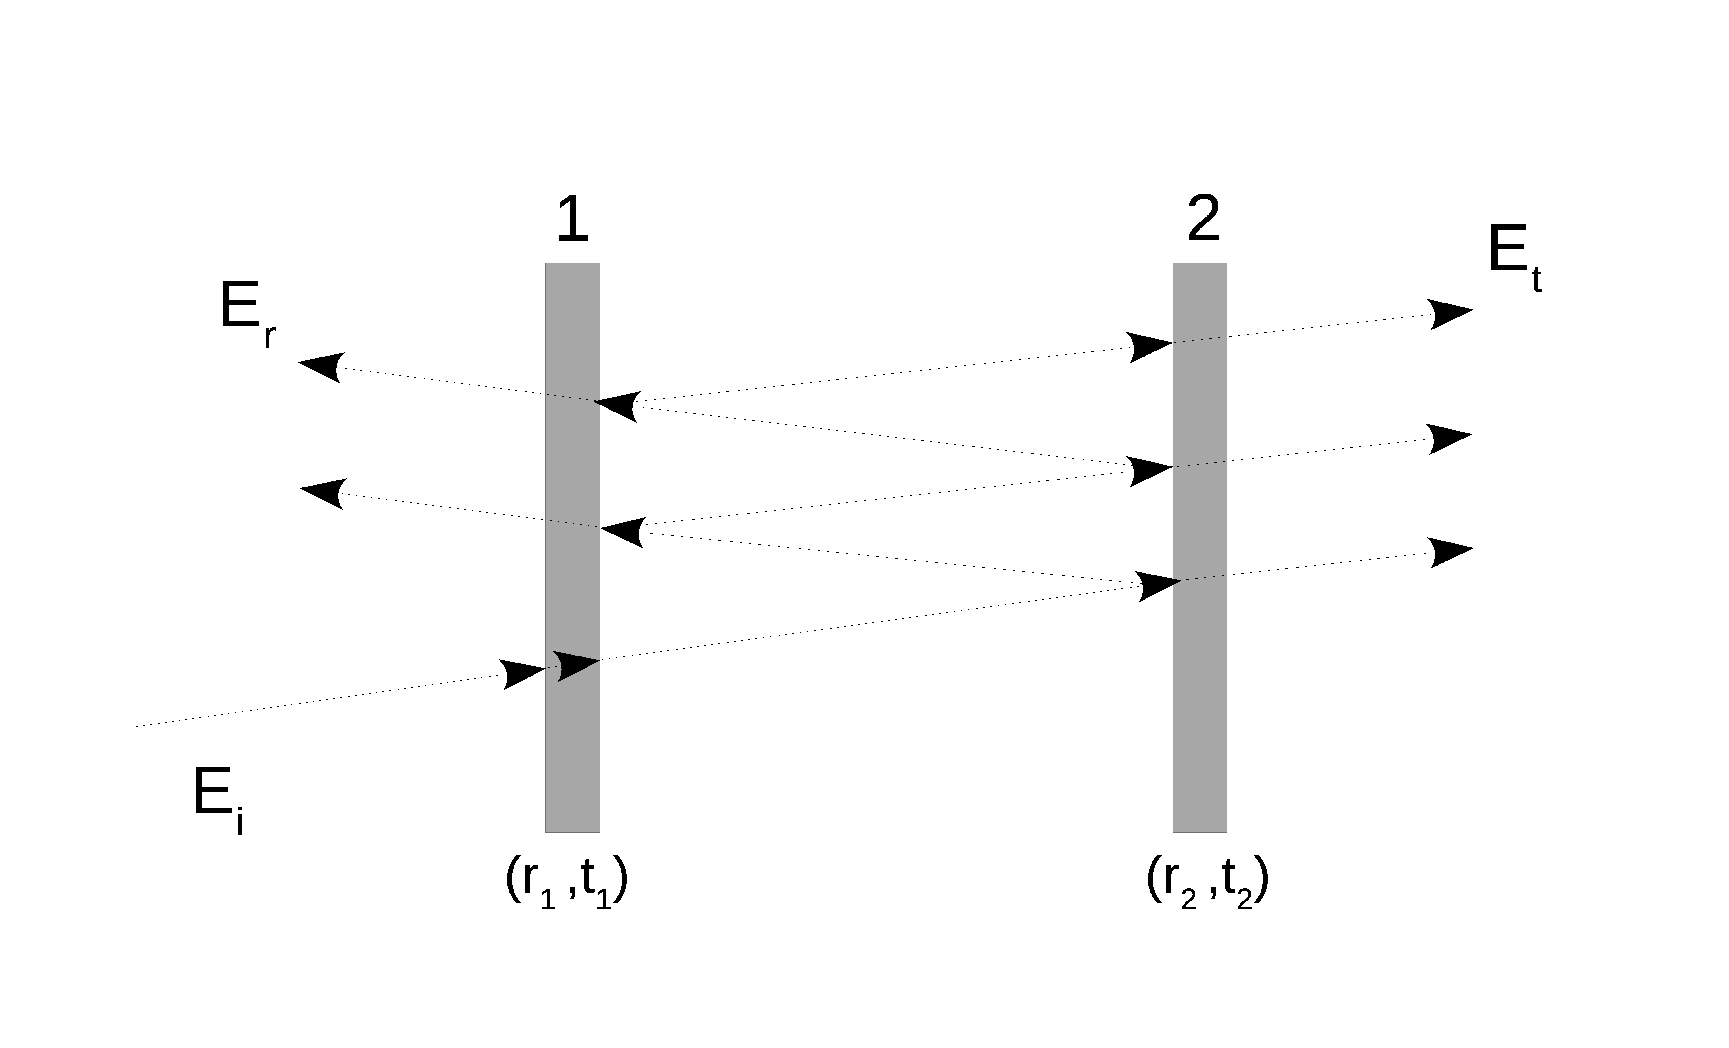
\includegraphics[width=0.60\textwidth]{Fabry_Perot_resonator.eps}
\caption{Illustrated energy diagram of a simple Fabry-Perot resonator}
\end{figure}



\newpage

\subsection{Theory of Fabry-Perot Interferometer}
 If the incident energy is in the form of white coherent light then at that point the transmission and reflection coefficients depend just on the mirror reflectivities. The total reflected power comprises of the power reflected from the principal mirror in addition to all the different reflections between the mirrors that add to the reflectivity in general. In summation, the equations are[1]: 
\begin{equation}
{\mathcal R} = R_{1} + T_{1}^2 R_{2} \sum_{m=1}^{\infty} (R_{1}R_{2})^{m-1} = \frac{R_{1} - 2R_{1}R_{2} + R_{2}}{1 - R_{1}R_{2}} _{\overrightarrow{R_{1} = R_{2} \equiv R}} \frac{2R}{1+R}
\end{equation}

Similarly, the transmitted energy in summation is:
\begin{equation}
{\mathcal T} = T_{1} T_{2} \sum_{m=1}^{\infty} (R_{1}R_{2})^{m-1} = \frac{T_{1} T_{2}}{1 - R_{1}R_{2}} _{\; \overrightarrow{R_{1} = R_{2} \equiv R}} \; \frac{T^{2}}{1-R^{2}} = \frac{1-R}{1+R}
\end{equation}

Assuming, be that as it may, the incident light comprises of a transiently lucid (monochromatic) plane wave, at that point the reflected power will be relative to the square of the reasonable total of every reflected field. Since the fields convey phase information with amplitudes added, the division of reflected and transmitted light depends not just on the mirror reflectivities but in addition on the mirror separation and excitation wavelength. The rational total of fields is amplified when every one of the fields interferes constructively (in phase) and limited when they interfere destructively (out of phase). Phase gathers with propagation separation as $\phi(z) = \beta z$ and may likewise be gained upon communication with the mirrors. The sound forms of Eqs. 2.1 and 2.2 incorporate an aggregated stage factor for each round-trip that can be translated as a standardized detuning $\phi = T_{R}\omega$, where $T_{R}$ is the cavity travel time, $T_{R} = n_{eff}L/c$ for the circumference, L and effective index $n_{eff}$. Presently, $\tilde{r}$ speaks to the complex reflectivity: 

\begin{multline}
\tilde{r} = r_{1} - t_{1}^{2}r_{2}\exp(i m \phi) \sum_{m=1}^{\infty} (r_{1}r_{2}\exp(i m \phi))^{m-1} \\ = \frac{r_{1} - r_{2}\exp(i \phi)}{1 - r_{1}r_{2}\exp(i \phi)} _{\; \overrightarrow{r_{1} = r_{2} \equiv r}} \; \frac{r(1-\exp(+i \phi))}{1-r^{2}\exp(+i \phi)}
\end{multline}

and $\tilde{t}$ represents the complex transmittivity:

\begin{multline}
\tilde{t} = -t_{1}t_{2}\exp(i m \phi/2) \sum_{m=1}^{\infty} (r_{1}r_{2}\exp(i m \phi))^{m-1} \\ = \frac{-t_{1}t_{2}\exp(i m \phi/2)}{1 - r_{1}r_{2}} _{\; \overrightarrow{r_{1} = r_{2} \equiv r}} \; \frac{-(1-r^{2})\exp(im \phi/2)}{1-r^{2}}
\end{multline}


The square modulus of these perplexing amounts gives the reflection ${\mathcal R}$ and transmission ${\mathcal T}$ coefficients (shown in Fig. 2.2). Antiresonant wavelengths are more emphatically reflected than in the ambiguous case, while resonant wavelengths are transmitted $100\%$ for adjusted reflectors ($r_{1}$ = $r_{2}$). For a fixed reflect dispersing, the transmission and reflection spectra in this manner show intermittent pinnacles and valleys. Figure 2.2 presenting the transmission and reflection spectra for a lossless, adjusted Fabry– Perot resonator. The part of reflected and transmitted power for mixed up excitation is identical to the separate spectrally averaged reflection and transmission over time of the spectrum range.

The values of reflectivity coefficients $r_{1}$, $r_{2}$ and the transmitivity coefficients $t_{1}$, $t_{2}$ are mentioned in the figure. The plot is of the intensity of the Fabry- Perot resonator versus the round trip phase of the system. This displays a $100\%$ transmission and $0\%$ reflection on the resonant frequencies. Meaning all the incident light is detected on the other side of the resonator of these specific frequencies. 

\begin{figure}[h]
\centering
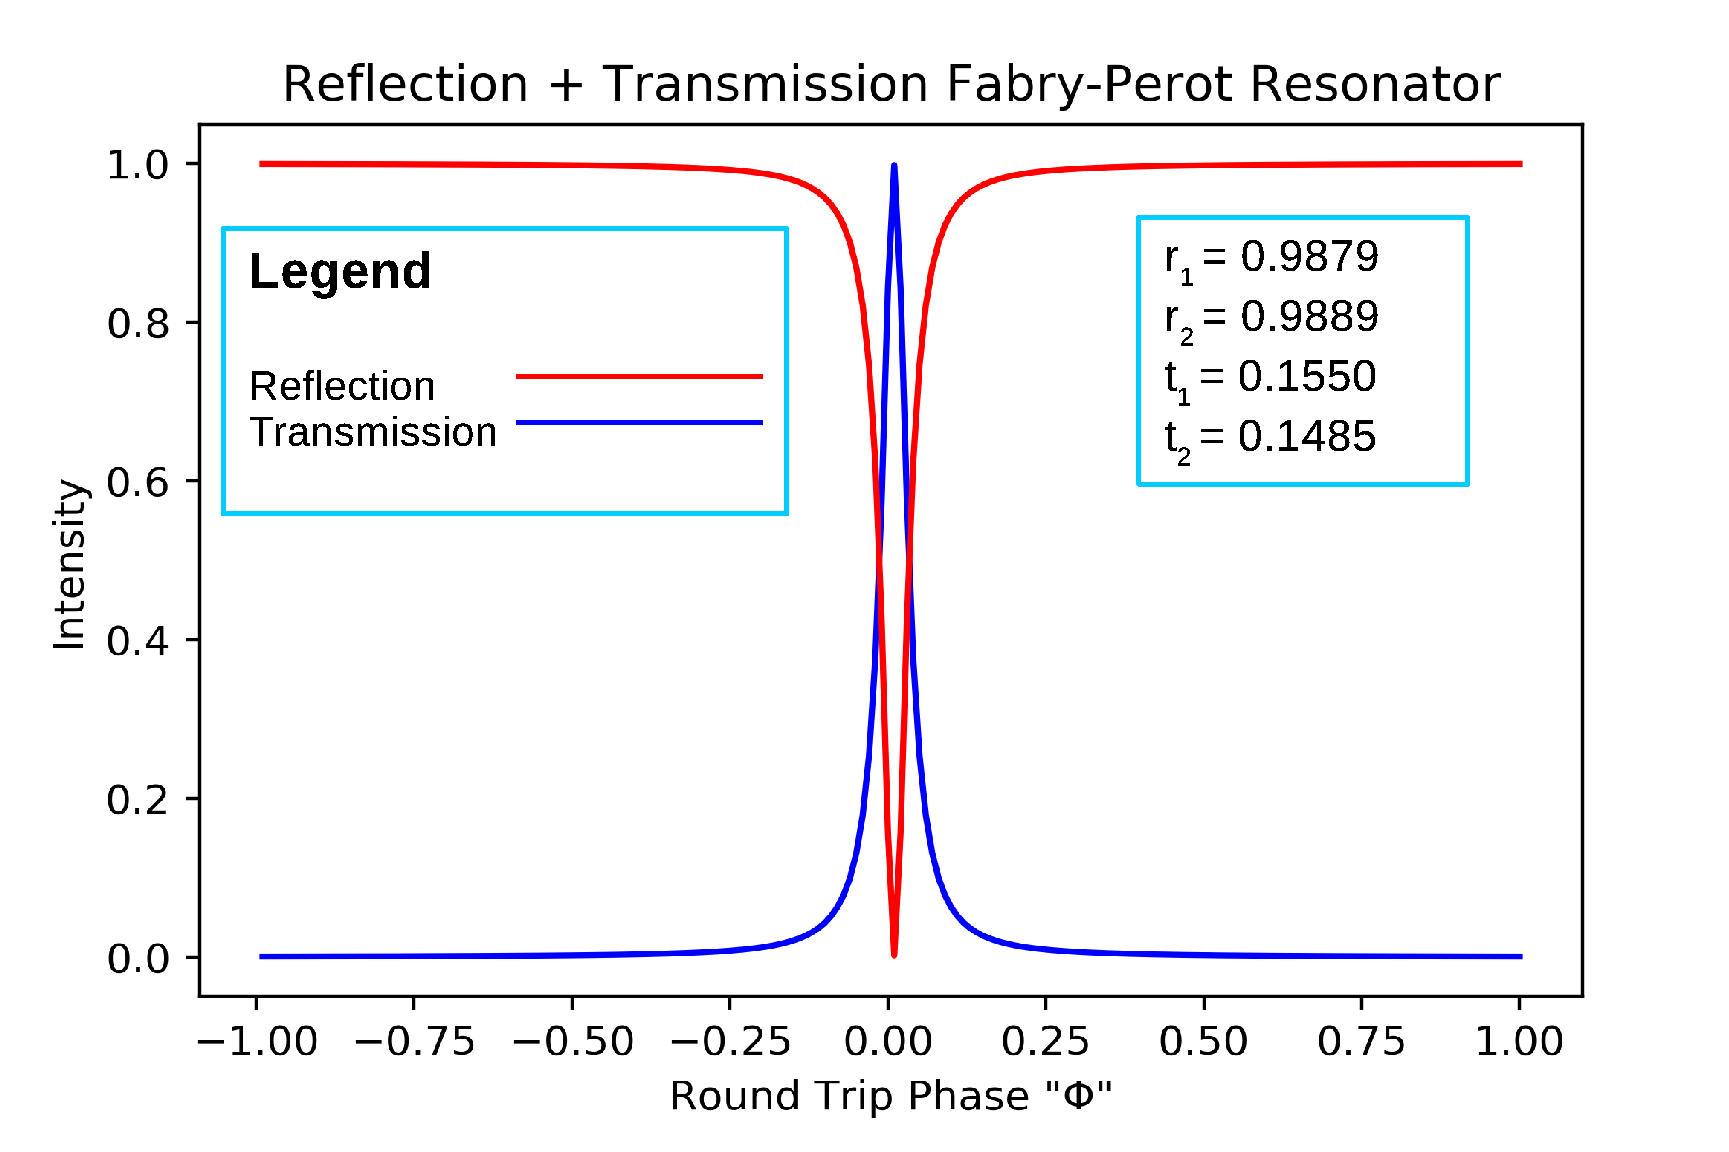
\includegraphics[width=0.85\textwidth]{R+T_FabryPerot.eps}
\caption{Transmitted and reflected field of an asymmetric Fabry-Perot resonator}
\end{figure}


\subsection{Effective Phase}
Now let us look at the phase details of the transmission and the reflection spectra of the asymmetric Fabry-Perot resonator. The phase gives us a lot of details about the traveling light inside the resonator and gives other details about dispersion, group delay, and group index. Fig. 2.3 shows phases of both transmission and reflection of an asymmetric Fabry-Perot resonator.

\begin{figure}[h]
\includegraphics[width=0.5\textwidth]{Phase_trans_FP.png}
\includegraphics[width=0.5\textwidth]{Reflec_Phase_FP.png}
\caption{Transmission and Reflection phase vs normalized detuning of an asymmetric Fabry-Perot resonator critically coupled.}
\end{figure}

The effective phase also called transmission phase of the system, which is the phase acquired upon transmission, gives us the information about the dispersion of the system. It is basically the argument of the complex transmitivity of the resonator (Eq. 2.4). Any complex number, $z = x + iy$, can be written as $z = |z|exp(i\phi)$. Where, $\phi$ is the argument of the complex number $z$ given by $\phi = tan^{-1}(y/x)$. Now we can write for our complex transmitivity as,

\begin{align*}
\frac{E_{t}}{E_{i}} = |\frac{E_{t}}{E_{i}}|\,exp(i\phi_{eff})
\end{align*} 

Where,

\begin{equation}
\phi_{eff} = arctan(\frac{Im[E_{t}/E_{i}]}{Re[E_{t}/E_{i}]})
\end{equation}

\subsection{Phasor Plots}
Phaser plots are another useful way to study the behavior of light inside the optical cavity. The phasor plots are the complex plots between Real and Imaginary parts of the complex reflectivity and transmitivity (equation 2.3 and 2.4 respectively). Figure 2.4 shows the phasor plots of both transmitivity and reflectivity of an asymmetric Fabry-Perot resonator over the detuning period of 0 to $2\pi$ radians. 

\begin{figure}[h]
\includegraphics[width=0.5\textwidth]{Trans_ImagvsReal_Phaser.png}
\includegraphics[width=0.5\textwidth]{Reflection_ImagvsReal_Phaser.png}
\caption{Phaser plots of complex Transmitivity and Reflectivity of an asymmetric Fabry-Perot resonator from 0 to $2\pi$}
\end{figure}

\subsection{Finesse, Q-factor}
\subparagraph{\normalfont \large The resonance condition is fulfilled when the (compelling) circumference of the ring, or for the most part the round-trip length, is equivalent to a whole number numerous of the optical wavelength inside the medium. This means a progression of Lorentzian-molded transmission bends equally dispersed in recurrence by the FSR (Free Spectral Range), with the resonance linewidth portraying the capacity time of photons inside the cavity. The photon lifetime can be standardized to one optical cycle, known as the quality factor (${\mathcal Q}$), or the cavity round-trip time, known as the cavity Finesse (${\mathcal F}$). The most extreme reachable Q-factor is characterized as ${\mathcal Q_{int}}$, which is the intrinsic loss of the cavity such that, ${\mathcal Q_{int}} = 2\pi\,n/(\alpha_{i}\,\lambda_{res})$ [16] where $\alpha_{i}$ is the intrinsic loss coefficient and $\lambda_{res}$ is the free-space resonant wavelength.  At the point when the resonator is coupled to the outer world, the Q-factor further decreases because of the loss imported by the coupler (${\mathcal Q_{ext}}$). This Q-factor, which defines mostly coupling and related external losses, can be given by ${\mathcal Q_{ext}} = (2n \pi L)/ {\lambda_{res}\, T}$, where $L$ is the circumference of the resonator (in case of a ring), $\lambda_{res}$ is the resonant frequency, and $T$ is the transmitivity coefficient. Thus the total quality factor ${\mathcal Q_{load}}$ is comprised of these two parts: ${\mathcal Q_{load}^{-1}}$ = ${\mathcal Q_{int}^{-1}}$ + ${\mathcal Q_{ext}^{-1}}$.}

\begin{align*}
{\mathcal F}inese = \frac{2 \pi}{\gamma} \\ 
\\
{\mathcal \gamma} = \frac{4}{\sqrt{F}} \\
\\
F = (\frac{2r}{1-r})^{2} 
\end{align*}

Thus,

\begin{equation}
{\mathcal F}inese = \frac{\pi \sqrt{F}}{2}
\end{equation}

Similarly, 

\begin{align*}
{\mathcal Q}_{factor} = \frac{\lambda_{res}}{FWHM} \\ 
\\
{\mathcal Q}_{factor} = \frac{nLf}{\lambda}
\end{align*}
\begin{equation}
{\mathcal Q}_{factor} = m f
\end{equation}


\section{Ring Shaped Resonators}
Optical interferometers such as Fabry-Perot or Gires-Tournois resonators are extremely useful in making devices that are compatible in making spectroscopy tools, add-drop filters for specific optical frequencies, laser cavities as well as dispersion compensators. Due to their free space structural design, they are quite incompatible with planar integrated technology. Thus, we require another geometry of devices which have similar spectral properties. These can be fabricated easily and effectively on microchips and waveguiding geometries by molding of different waveguides into a ring shape.

Let us now discuss how to ring resonators, whose principle is pretty much similar to the Fabry-Perot resonator and are more simple to make, operate. Basically, a ring resonator is a simple waveguide which is turned in the shape of a ring (see Fig. 2.5). This allows it to exhibit resonant behavior on very specific frequencies.


\subsection{Evanescent Coupling}
The optical systems discussed above experiences the passage of light across the ring from the optical waveguide through a process known as evanescent coupling. Evanescent coupling is a classical phenomenon whose quantum interpretation is exactly as photon tunneling. It is basically the power transfer of the wave which is directly dependant on the proximity of the bent waveguide and from the straight waveguide. Also, the length or area that has been exposed to the coupler also plays an important role in i.e how many parts of the waveguide/resonator overlaps; illustrated in Fig. 2.5.
\subparagraph{\normalfont \large Coupling strength of an ideal coupler is dependant on the interaction length between the two optical modes which means that the power will transfer more efficiently when the two modes are matched on the basis of their respective phases. This allows us to observe distinct behaviors as well as multiple resonances in transmittance and reflectance.} 

\begin{figure}[h]
\centering
\includegraphics[width=0.50\textwidth]{evanescent_wave.png}
\caption{Schematic illustration of the microsphere-fiber-taper
system.[2]}
\end{figure}

\subparagraph{\normalfont \large The light is coupled inside the ring due to two sets of coupling approaches, one being lateral and other being vertical. Either one of these two approaches is necessary for the light from the optical waveguide to couple inside the bent waveguide (ring). The light stays, or resonates, inside the bent waveguide due to the effect of total internal reflection. Lateral coupling requires the same plane fabrication of waveguide and bent waveguide which are easier to fabricate. To ensure strong coupling, small separation is required between the waveguide and bent waveguide. Lateral configuration requires a single layer only but very accurate lithography and etching processes must be done to open up the gaps between straight and ring waveguides with high precision. In vertical coupling transport and bent waveguides are etched in various layers. Vertical coupling expels the index contrast restriction of lateral coupling, additionally, it is an empowering innovation for the ring radii less than $ \approx5 \mu m$. Another bit of leeway of the vertical arrangement is that the ring and waveguide layers don't need to be a similar thickness, which improves the design opportunity.}


These resonators, when fabricated on the chip, display different effects of coupling and transfer of wave energy. These kinds of behaviors have been noticed in all kind of classical waves, such as sound waves, which was first observed inside a large cathedral's halls, thus it was named whispering gallery modes [4]. Also, these resonators can be made using different material but in the scope of this thesis, we used semiconductor silicon as the primary material. 


\subsection{Coupling Regimes}

The transmission spectrum of the waveguide-ring coupled system now depends on the proximity and coupling effects. Let us discuss different coupling conditions for these resonators. Fig. 2.11 shows plots for an all-pass resonator for under, over, and critically coupled system and also for a lossless all-pass system.

\begin{figure}[h]
\centering
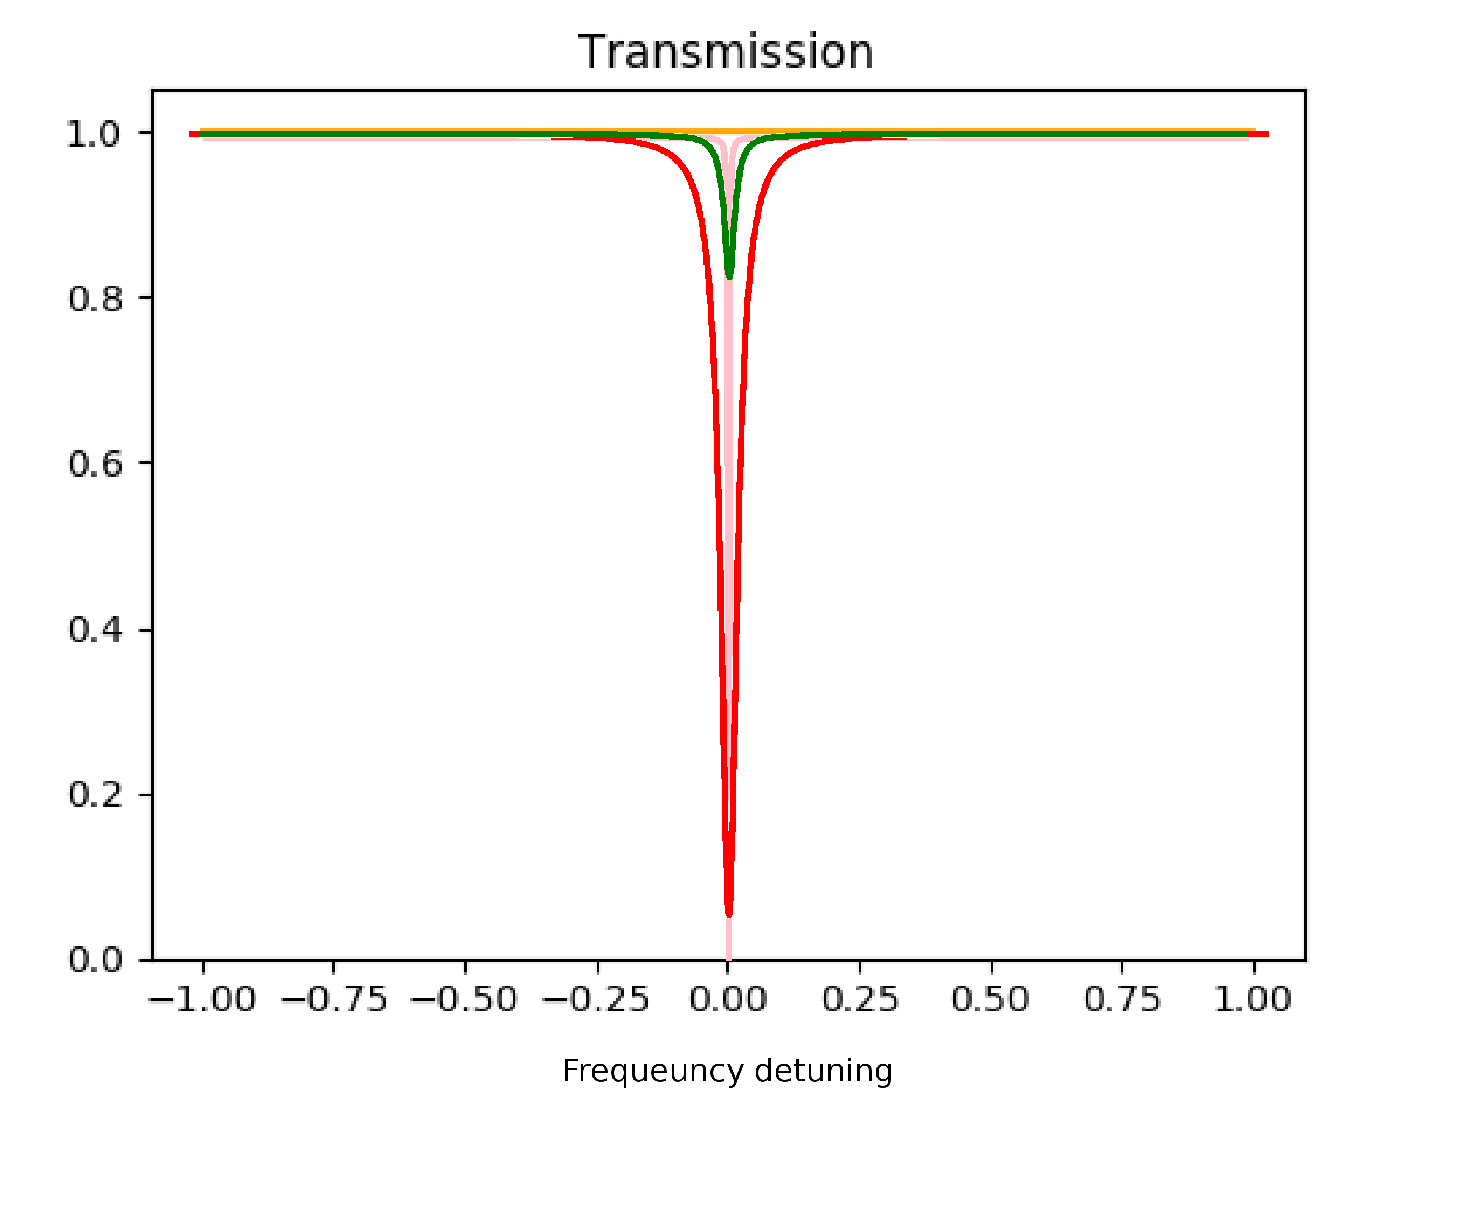
\includegraphics[width=0.5\textwidth]{under_over_couple.eps}
\caption{Different couplings shown in different colors.}
\end{figure}

Light when couples inside the ring will lose some part of its intensity. The amount of light that travels inside the ring will acquire a phase shift by completing one round trip and will now interfere destructively with the light which was not coupled inside the resonator. If the phase shifted light has amplitude weaker than the original or uncoupled light, the regime will be known as under-coupled. If the amplitude is higher than the original pulse, the regime would be over-coupled. Similarly, when the amplitude matches exactly with the outside light, the regime would be known as critically coupled. Also, if the light passes through the system without any attenuation or loss, we get $100\%$ transmission.


\section{Gain Incorporation in Resonators}
Light, when travels through a medium, loses its intensity exponentially. This effect can be explained by Beer's Law for electromagnetic intensity. But some mediums, whose refractive index is such as they oppose the exponential decay of the light and rather increase the intensity in the propagation through the medium, are called natural gain medium. Also, there can be an artificial source to activate gain in a certain system. This is done by pumping energy or external light source i.e. Lasers, to excite the atoms inside the cavity. This makes the stimulated emission releases of the photons increase exponentially and we see an increase in the incident intensity of the input light. We can use these gain mediums and build micro-resonators from them and observe different quantum optical phenomenons. First I will explain a bit about how gain works.


\subsection{Beer's Law}
The simple radiation law follows the beer's law in the absorption of any kind of radiation inside a medium. This tells us that the initial intensity of the light source depends on the variables of the medium it is passing through. For electromagnetic radiation, we can write this law as,

\begin{equation}
I(z) = I_{o}\exp(-\alpha z)
\end{equation}

Here, $I_{o}$ is the initial intensity of the radiation, $\alpha$ is the attenuation constant of the medium, $z$ is the amount of distance traveled through the medium and $I(z)$ is the intensity of light after traveling the distance $z$.

\begin{figure}[h]
\centering
\includegraphics[scale=0.75]{beer's_law_withoutgain.png}
\caption{Beer's law plot with attenuation 0.01/cm: y-axis shows the intensity of light and x-axis shows the distance traveled in meters.}
\end{figure}


\subsection{Beer's Law in Presence of Gain}
In a gain medium, the intensity of the light will not decrease but it will gradually increase. This means that the attenuation $\alpha$ is negative or we can introduce a new coefficient for such medium say $g$ such that $-\alpha \to +g$ where $g$ is some positive real number. This means that the intensity function now grows exponentially rather than decaying exponential.

\begin{equation}
I(z) = I_{o}\exp( +g z)
\end{equation}

\begin{figure}[h]
\centering
\includegraphics[scale=0.75]{beer's_law_withgain.png}
\caption{Beer's law plot with gain value 0.01/cm: y-axis shows the intensity of light and x-axis shows the distance traveled in meters.}
\end{figure}

\subsection{Gain Medium}
The active laser medium also called gain medium or lasing medium is the source of optical increase inside a laser. The gain is the result of stimulated emission of electronic or sub-atomic changes to a lower energy state from a higher energy state recently populated by a pump source. This gain in optical systems is usually used for amplification purposes and hence make optical amplifiers. Certain crystals, typically doped with rare-earth ions (e.g. neodymium, ytterbium, or erbium) or transition metal ions (titanium or chromium) can be used as a gain medium. Also, Semiconductors, e.g. gallium arsenide (GaAs), indium gallium arsenide (InGaAs), or gallium nitride (GaN) can also be used when doped [14]. Also, some material such as liquids in the form of dye solutions as used in dye lasers can also be used to make a gain element for active resonators [15].


\section{Group Delay and Group Advance}
The velocity of light is a universal constant $c \approx 299792458 m/s$ in free space. However, the light velocity depends upon the medium when it propagates through it. The medium's dispersive properties are defined by the refractive index $n$ of the material. The light pulse propagating from this material experiences delay in the arrival time as compared to the arrival time in a vacuum. 
To comprehend the results of scattering of the refractive index, we initially think about the proliferation of monochromatic light emission through a material. The phase velocity ($v_{p}$) depicts the speed at which the wavefronts travel through the material and is given by: $v_{p} = c/n $ . Thus when the light pulse propagates through the medium, each component of the wave travels at different speed because $n$ is a function of frequency $\omega$. Here, group index is put into account due to the collective effects upon the wave packets of different frequencies, which is given by:
\begin{align*}
n_{g} = n + \omega\frac{dn}{d\omega}
\end{align*}

Here, $n_{g}$ is the group index of the material and $\omega$ is the frequency of the wave. Thus now we can define the group velocity of the propagating wave, which is the speed at which the envelope of the incoming pulses moves through the dispersive medium, given by:
\begin{align*}
v_{g} = \frac{c}{n_{g}}
\end{align*}

Thus the reduction of the light experience in its velocity inside a dispersive medium. If the value of $n_{g} \approx 10^{8}$, then we experience ultra slow velocities of light which are measured up to $8m/s$ [17-19]. If group index becomes less than 1, such that $n_{g} < 1$, then we observe group velocities greater than the speed of light in vacuum, such that, $v_{g} > c$. This does not violate Einstein's Theory of Relativity [20] because there exist various proposals [5–8] for observing such effects by using anomalous dispersion near an absorption or gain lines [7-8]. The group index can also become negative, such that $n_{g} < 0$, resulting in negative group velocities which are sometimes also referred as 'Backward light' because it appears to propagate backward in the medium. We can understand the negative group velocity by having a medium of length $d$, so it will take $d/v_{g} = n_{g}d/c$ amount of propagation time for a light pulse to cross it. And the vacuum transition time would be $d/c$, thus the time delay would be $\Delta T = d/v_{g} - d/c$ which can be written as, $(n_{g}-1)d/c$. So for negative values of $n_{g}$, the delay time $\Delta T$ is negative which results in group advancement. This concept can be perceived as that if the light pulse is incident on such medium, the light pulse would appear on the other side sooner than if it had traveled through a vacuum. Figure 2.8 illustrates the propagation through a negative index medium [9]. 

\begin{figure}[h]
\centering
\includegraphics[scale=0.75]{negative_vg_pic.pdf}
\caption{Time intervals of a wave propagating through a negative index material. Notice that the peak of entering pulse leaves before it enters the system.}
\end{figure}

The slow light propagation of light is enhanced by EIT which is a transparency window in the absorption line of the system. Slow light can be used in optical buffers where controllable slow light can dramatically increase the system's performance. Also, the spectral sensitivity of an interferometer [11] can be highly enhanced by introducing a slow-light medium, as well as slow light has a large number of uses in defense applications. Fast light, on the other hand, can be used to make ultra-sensitive gyroscopes [12] and gravitational wave detectors in the fields of astrophysics [13].



\section{All-Pass Ring Resonator}
A straightforward ring resonator is made by taking one yield of a conventional directional coupler and bolstering it once again into one input. Such a device displays periodic cavity resonance (reverberation) when light navigating the ring procures a phased move relating to a number numerous of 2$\pi$ radians. The resonator is numerically defined from two parts: a coupling quality and an input way. In opposition to the limitless entirety inferences performed before for the Fabry– Perot and Gires– Tournois, in which we expected steady-state task and coordinating fields and derived basic spectral properties. Although both strategies are similarly substantial, the field-coordinating technique has the benefit of simplicity.
\begin{figure}[h]
\centering
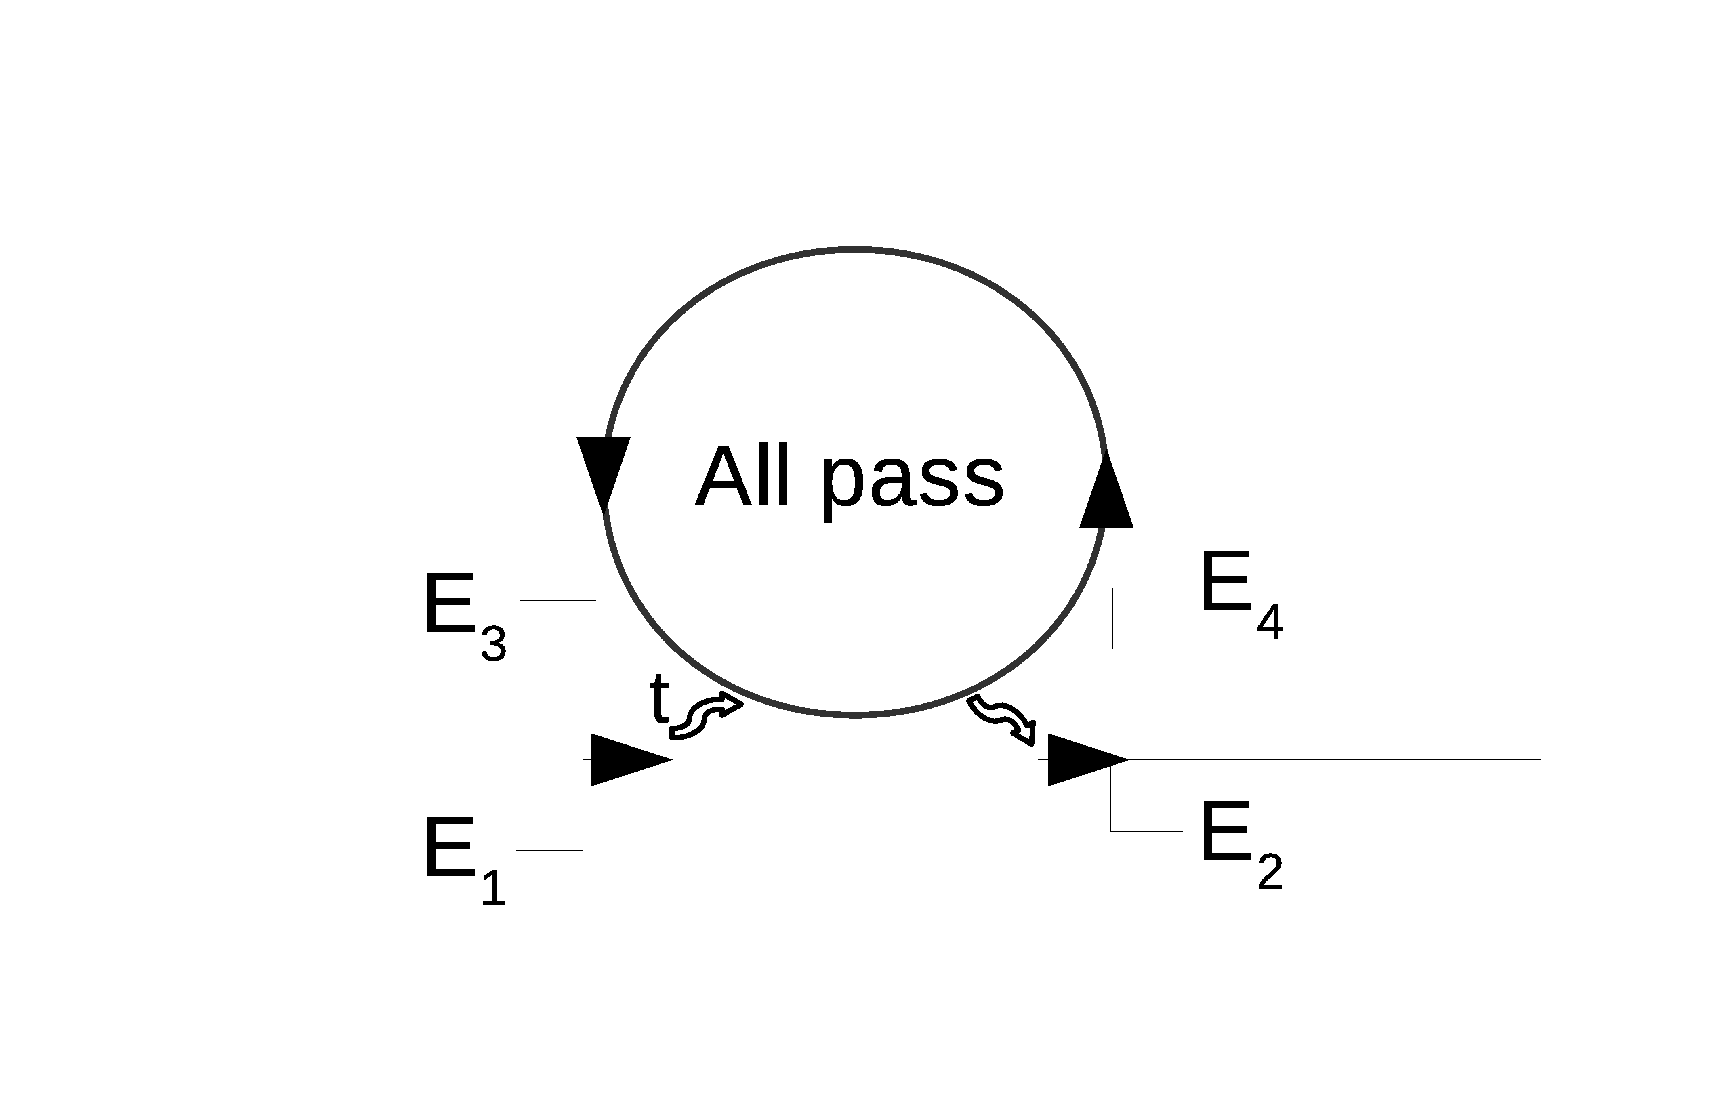
\includegraphics[width=0.85\textwidth]{all_pass_resonator.eps}
\caption{Illustrated fields of an all-pass resonator}
\end{figure}

Fig. 2.9 illustrates the basic geometry of the all-pass ring resonator with its respective energies. The incoming input power is $E_{1}$, which couples inside the ring through the evanescent coupling. Then it travels as energy $E_{4}$ and makes a round trip phase. If this phase matches with the input signal, it makes constructed interference with the incoming light with energy $E_{3}$ and transfers its energy to the optical waveguide again with energy $E_{2}$. The complex transmitivity and reflectivity are given by equation 2.10, as the reflection is not considered in this geometry.
 

\begin{equation}
\frac{E_{t}}{E_{i}} = \frac{r - a_{1} e^{i\phi_{1}}}{1 - r a_{1} e^{i\phi_{1}}}
\end{equation}

Here, $r$ is the self-coupling coefficient, $a = e^{-\alpha L/2}$ is the intrinsic loss for circumference $L$ and attenuation $\alpha$, and $\phi = \omega T$ is the round trip phase of the ring or single pass phase shift.

\subsection{Transmission For Passive and Active}
Let us look at the transmission spectra of the passive and active all-pass ring resonator. Fig. 2.10 shows that the transmission peak is changed into a dip as was in the case of a symmetric Fabry-Perot resonator. On the right, it shows when the gain is introduced inside the system, the dip flips into a peak above the 1 mark on the graph telling us that we have more transmission on resonant frequencies than the actual input.
\begin{figure}[h]
\includegraphics[width=0.5\textwidth]{trans_ring_withoutgain.png}
\includegraphics[width=0.45\textwidth]{all-pall_gain.png}
\caption{Transmission spectra of a passive All-pass ring resonator}
\end{figure}


\subsection{Effective Phase}
The phase of the All-pass ring resonator is shown in Figure 2.12. We can easily observe from this that with changing the values of the coupling $r$, the shape of the graph changes as that of a function of $ArcTan(\phi)$. The relation for phase is given by,
\begin{equation}
\Phi_{eff} = \pi + \phi + 2\tan^{-1}\frac{r\sin\phi}{1-r\cos\phi}
\end{equation}

\begin{figure}[h]
\centering
\includegraphics[width=0.65\textwidth]{allpassphase_new.png}
\caption{Phase diagram of an All-Pass ring resonator from 0 to $\pi$ where $r$ is the coupling parameter.}
\end{figure}

\subsection{Phasor Plots}
Now looking into some complex transmitivity of an All-pass ring resonator (Fig. 2.13). This plot is plotted over the complex plain of the detuning limits from 0 to 2$\pi$. 

We observe that the transmission loop does not go to the negative real axis and touches exactly on the origin. The loop cuts the real axis twice on 0 and 1 and is symmetric above and below the axis. 
\begin{figure}[h]
\centering
\includegraphics[width=0.5\textwidth]{Imag_vs_real_allpass.png}
\caption{Phaser plot of complex transmitivity of an all-pass ring resonator}
\end{figure}


\section{Add-Drop Ring Resonator}
The immediate waveguide similarity of a free-space Fabry– Perot is acquired by including a second guide that side-couples to the resonator.
Since this setup acts as a tight band abundancy channel that can include or drop a recurrence band from an approaching sign, it is usually named as an add-drop filter. Fig. 2.14 shows the basic geometry of the add-drop ring resonator with its associated fields labeled accordingly. This resonator has an input, through and drop interfaces where $t_{1}$ is add and $t_{2}$ is drop coefficients. Input field is labeled as $E_{1}$ while the through field is labeled as $E_{2}$. The drop field is on the left top corner labeled as $E_{5}$. The ratio of these fields to the incident/input field defines the total transmitivity and total reflectivity of the filter. The transmission and reflection relations are given in equation 2.12 and 2.13.
\begin{figure}[h]
\centering
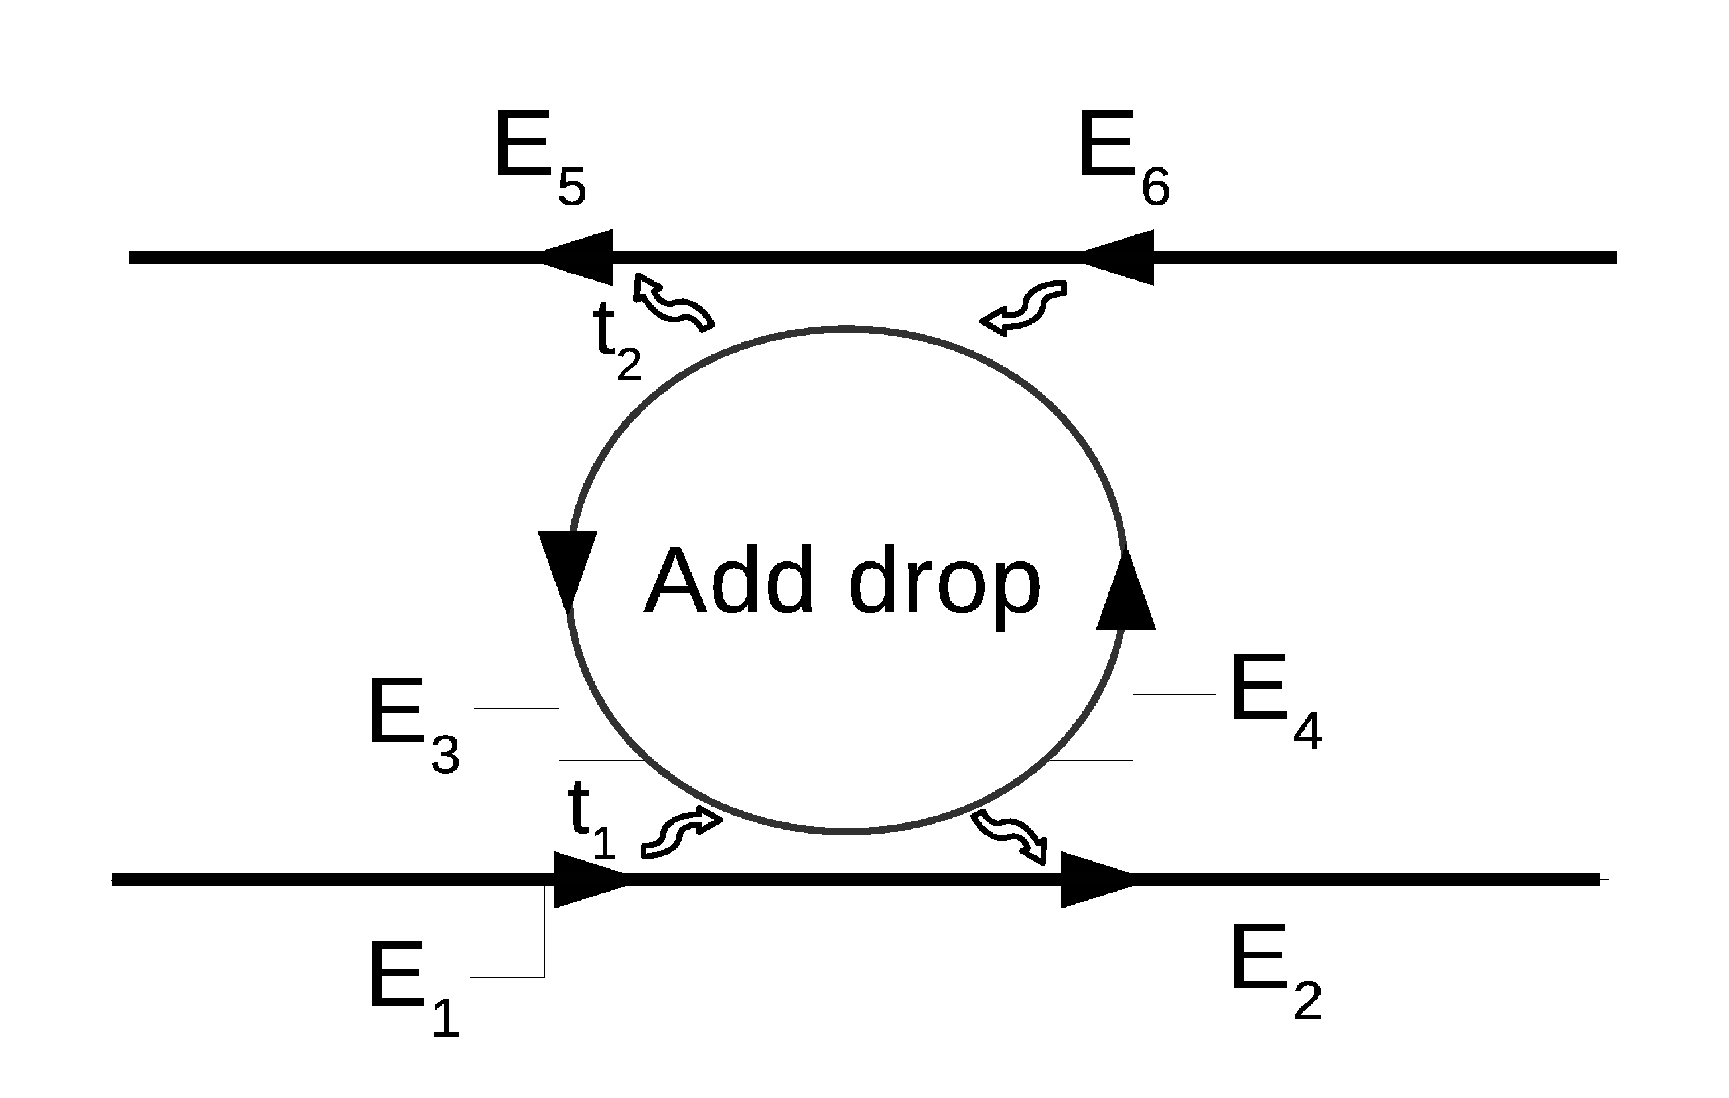
\includegraphics[width=0.70\textwidth]{add_drop_resonator.eps}
\caption{Illustrated fields of an add-drop resonator}
\end{figure}


\begin{equation}
\frac{E_{t}}{E_{i}} = \frac{r_{1} - r_{2} a_{1} e^{i\phi_{1}}}{1 - r_{1} r_{2} a_{1} e^{i\phi_{1}}}
\end{equation}

\begin{equation}
\frac{E_{r}}{E_{i}} = \frac{- t_{1} t_{2} a_{1} e^{i \phi_{1}/2}}{1 - r_{1} r_{2} a_{1} e^{i\phi_{1}}}
\end{equation}



\subsection{Transmission and Reflection}
Let us now look at some reflection and transmission spectra of a passive Add- drop filter. Fig. 2.15 shows that the transmission and reflection peaks are flipped as in case of an asymmetric Fabry-Perot resonator and the transmission phase is a direct function of the detuning. Reflection phase is also shown in Fig. 2.16.

\begin{figure}[h]
\centering
\includegraphics[width=0.5\textwidth]{all_pass_plots_a.png}
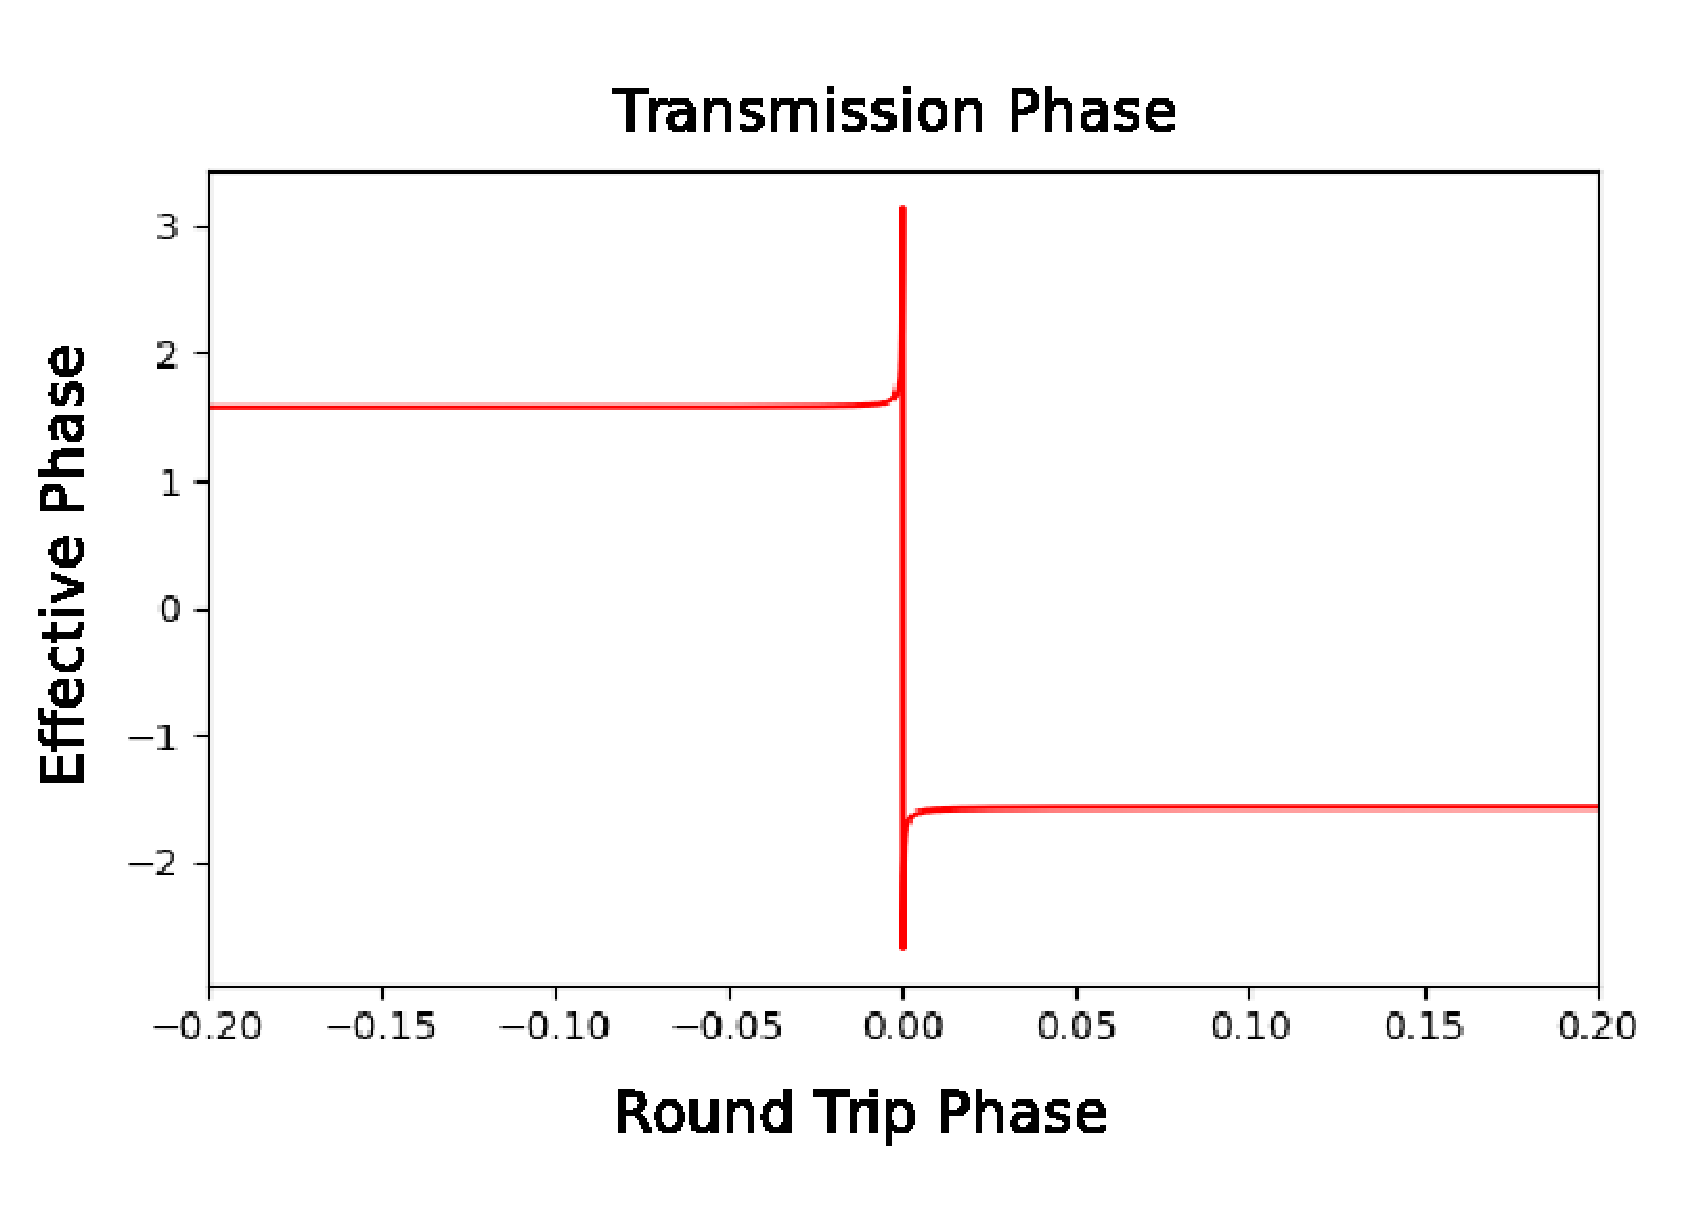
\includegraphics[width=0.5\textwidth]{all_pass_plots_a2.eps}
\caption{Reflection and Transmission spectra along with transmission phase} 
\end{figure}
\newpage
\begin{figure}[t]
\centering
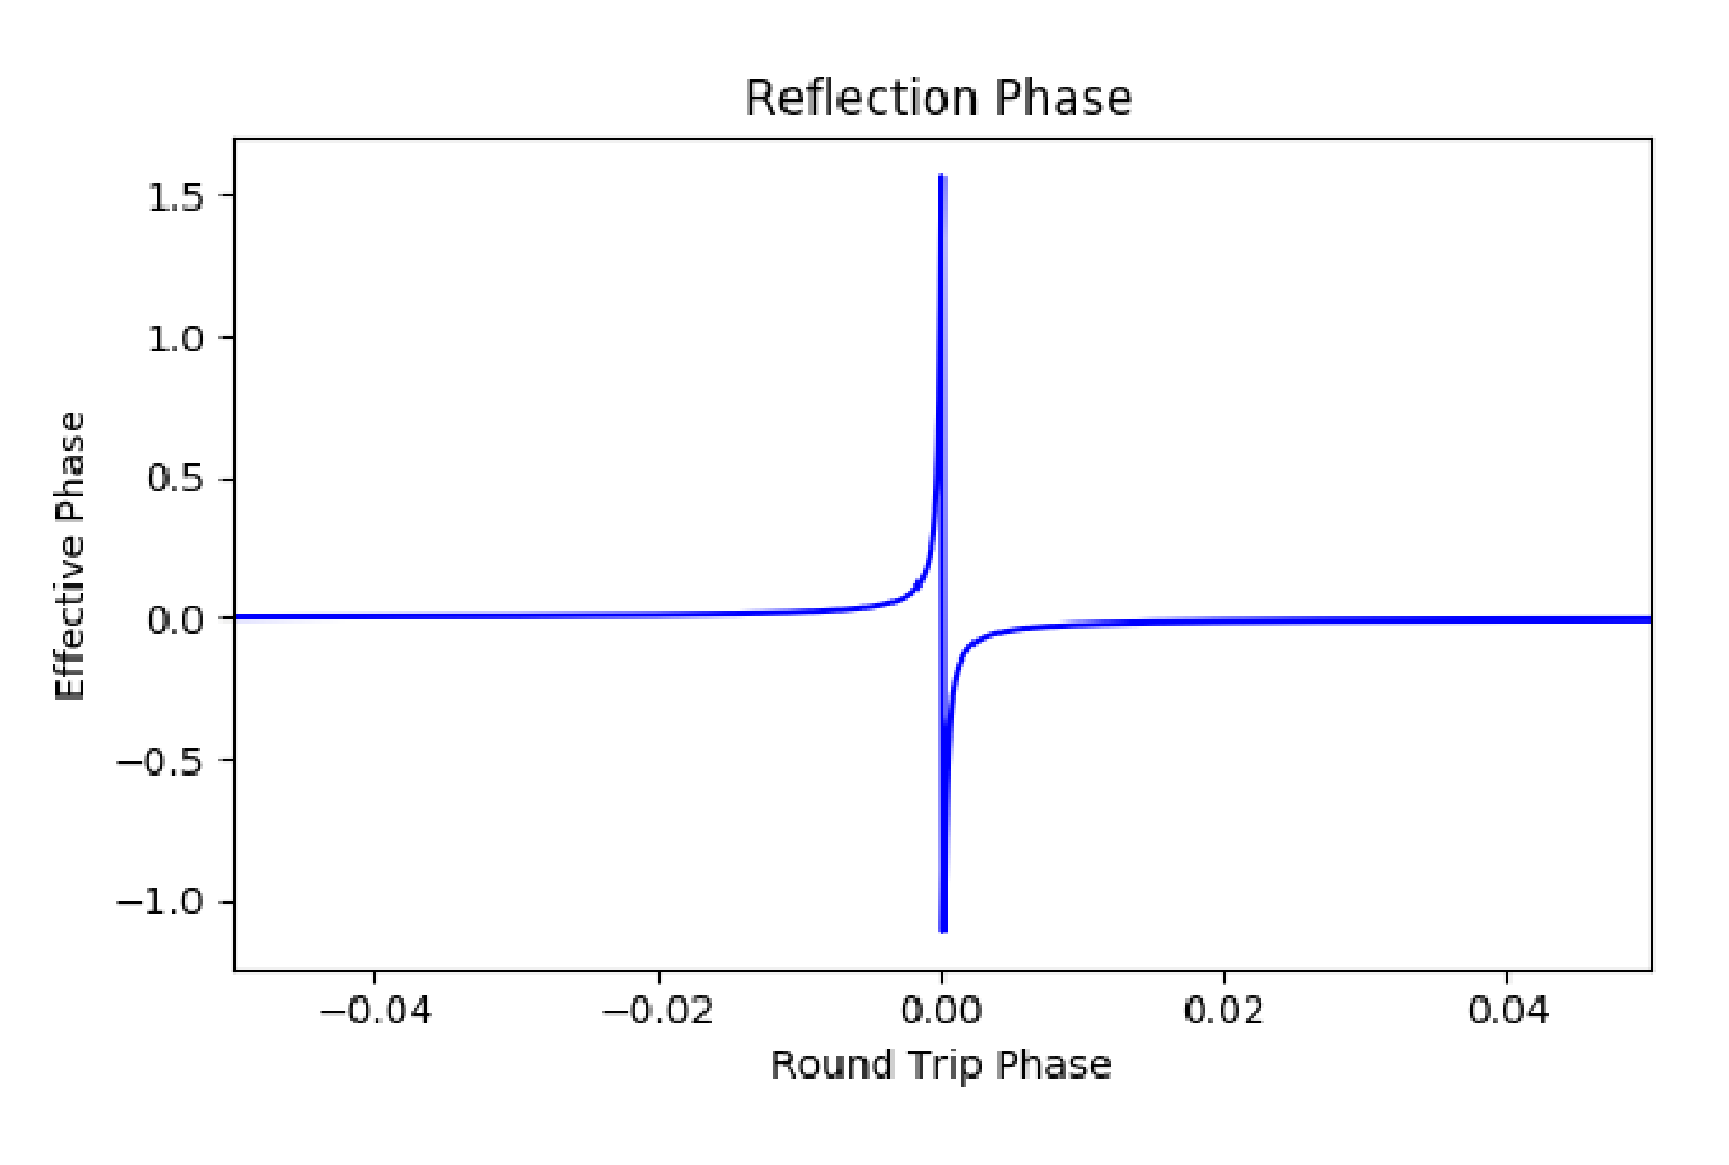
\includegraphics[width=0.5\textwidth]{all_pass_plots_b.eps}
\caption{Reflection phase of the all-pass ring resonator.}
\end{figure}

\subsection{Transmission and Reflection with gain}
Now we introduce gain into the system and observe that the transmission dip also shifts into a peak which above the 1 mark (see Fig. 2.17). Meaning that it is greater than the initial intensity and the reflection peak is almost near zero meaning most of the incident light is being transmitted. We will study the transmission of some other different geometries of ring resonators with gain. 


\begin{figure}[h]
\centering
\includegraphics[width=0.85\textwidth]{add_drop_gain_plots.png}
\caption{Gain introduced into an all-pass resonator: we see clear difference in the intensities.}
\end{figure}

\subsection{Phasor Plots}
Now let us see how complex plots of Add drop is different from the All-pass resonator. Fig. 2.18 shows that the loop goes towards the negative real axis as the phase is increased. This tells a lot about the distinct behavior.

\begin{figure}[h]
\centering
\includegraphics[width=1\textwidth]{ImagVsReal(add-drop).png}
\caption{Phaser plots of complex Transmitivity and Reflectivity of an All-pass ring resonator from 0 to $2\pi$}
\end{figure}


\section{Two Coupled Ring Resonator}
Now we turn another optical waveguide into a ring shape and install it on the top of the all-pass ring resonator such that now we have dual ring geometry and a waveguide coupler. This geometry does allow resonant behaviors and the spectra vary largely from an all-pass resonator.
In this arrangement, the coupling between the two resonators (rings) also plays an important role in the spectra of the light that passes through the resonator. Fig. 2.19 displays the basic geometry of the couple ring system we are going to discuss along with their energies. The circumference of these resonators are same for both rings given by $b = 25\mu m$, and the refractive index for these resonators is $n=3.45$ and the Quality Factors are given as $Q_{1} = 1\times10^{5}$ and $Q_{2} = 1\times10^{6}$

\begin{figure}[h]
\centering
\includegraphics[width=0.65\textwidth]{couple_ring_resonator.eps}
\caption{Illustrated fields and geometry of a coupled ring resonator}
\end{figure}

In this geometry, we will study the transmittance of the system as the symmetric case is its reflection in every case. The equation for complex transmitivity of this two resonator system is,

\begin{equation}
\frac{E_{t}}{E_{i}} = \frac{r_{1} - r_{12} a_{1} e^{i\phi_{1}}}{1 - r_{1} r_{12} a_{1} e^{i\phi_{1}}}
\end{equation}

where $r_{12}$ is the coupling parameter of the second resonator and is also a complex number given by,

\begin{align*}
r_{12} = \frac{r_{2} - a_{2} e^{i\phi_{2}}}{1 - r_{2} a_{2} e^{i\phi_{2}}}
\end{align*}


\subsection{Coupled Resonator Induced Transparency and Absorption}
Coupled resonator systems, like the one above, have been observed to display the quantum interference effects like Electromagnetically Induced Transparency and Electromagnetically Induced Absorption (EIT and EIA) via their optical analog known as Coupled Resonator Induced Transparency and Absorption (CRIT and CRIA) [3,4]. These quantum interference effects are observed in atoms with at least 3 energy levels but the similar optical analogs of these effects can be seen in these classical resonator systems. This enables enhanced dispersion and transitions from superluminal and subluminal group velocities at room temperature and in micro level scale. These effects will be discussed in detail using ring geometry optical microresonators in later chapters.

\newpage
\section*{References}
\addcontentsline{toc}{section}{References}
\paragraph{\normalfont \large $[1]$ J. Heebner, R. Grover, T. Ibrahim “Optical Microresonators, Theory, Fabrication, and Applications", Springer Science+Business Media (2008)\\
\\ $[2]$ K. Totsuka and M. Tomita “Dynamics of fast and slow pulse propagation through a microsphere–optical-fiber system", Phy. Rev. E \textbf{75} (2007)\\
\\ $[3]$ D. D. Smith, H. Chang, K. A. Fuller, A. T. Rosenberger, and R. W. Boyd, “Coupled-resonator-induced
transparency,” Phys. Rev. A \textbf{69}, 063804 (2004)\\
\\ $[4]$ A. Naweed, G. Farca, S. Shopova, and A. T. Rosenberger, “Induced transparency and absorption in coupled
whispering-gallery microresonators,” Phys. Rev. A \textbf{71} (2005).\\
\\ $[5]$ C. G. B. Garrett, and D. E. McCumber, “Propagation of a Gaussian light pulse through an anomalous dispersion medium." Phys. Rev. A \textbf{1}, 305 (1970).\\
\\ $[6]$ Chu, S. and Wong, S. “Linear pulse propagation in an absorbing medium.“ Phys. Rev. Lett. \textbf{48}, 738
(1982).\\
\\ $[7]$ R. Y. Chiao, Superluminal (but causal) propagation of wave packets in transparent media with inverted atomic populations. Phys. Rev. A \textbf{48}, R34 (1993).\\
\\ $[8]$ E. Bolda, J. C. Garrison, and R. Y. Chiao, “Optical pulse propagation at negative group velocities due to a nearby gain line." Phys. Rev. A \textbf{49}, 2938 (1994).\\
\\ $[9]$ R.W. Boyd and D. Gauthier “Controlling the Velocity of Light Pulses", Science \textbf{326} (2009)\\
\\ $[10]$ L. J. Wang, A. Kuzmich and A. Dogariu “Gain-assisted superluminal light propagation", Nature \textbf{406} (2000)\\
\\ $[11]$ K. J. Vahala, “Optical microcavities,” Nature \textbf{424}, 839 (2003).\\
\\ $[12]$ Z. Shi, R. W. Boyd, D. J. Gauthier, C. C. Dudley, “Enhancing the spectral sensitivity of interferometers
using slow-light media” Opt. Let. \textbf{32}, 8 (2007).\\
\\ $[13]$  M. Salit, G. S. Pati, K. Salit and M. S. Shahriar “Fast-light for astrophysics: super-sensitive gyroscopes and gravitational wave detectors” Journal of Modern Optics \textbf{54}, 16 (2007).\\
\\ $[14]$\,  Hecht, Jeff. The Laser Guidebook: Second Edition. McGraw-Hill, 1992. (Chapter 18-21).\\
\\ $[15]$  F. J. Duarte and L. W. Hillman (Eds.), Dye Laser Principles (Academic, New York, 1990).\\
\\ $[16]$ A. Naweed, “Photonic coherence effects from dual-waveguide coupled pair of co-resonant microring resonators", Opt. Exp. \textbf{23} (2015).\\
\\ $[17]$ L. V. Hau, S. E. Harris, Z. Dutton, and C. H. Behroozi, “Light speed reduction to 17 meters per second in
an ultracold atomic gas." Nature \textbf{397}, 594 (1999).\\
\\ $[18]$ M. M. Kash, et al. “Ultraslow group velocity and enhanced nonlinear optical effects in a coherently
driven hot atomic gas." Phys. Rev. Lett. \textbf{82}, 5229 (1999).\\
\\ $[19]$ D. Budker, D. F. Kimball, S. M. Rochester, and V. V. Yashchuk, “Nonlinear magneto-optics and reduced group velocity of light in atomic vapor with slow ground state relaxation." Phys. Rev. Lett. \textbf{83}, 1767 (1999).
\\ $[20]$ A. Einstein, H. A. Lorentz, H. Minkowski, H. and Weyl, “The Principle of Relativity, Collected Papers"
(Dover, New York, 1952).}
 
\chapter{Coupled Resonators with Gain}
\section{Electromagnetically Induced Transparency}
Electromagnetically Induced Transparency (EIT) is a well-known phenomenon in quantum optics and its all-optical analog has generated tremendous interest in physics. EIT is a transparency window in the transmission spectrum. The narrow transparency window is the result of Fano-like interference among two transition pathways. There is another similar concept which is known as Autler-Townes Splitting (ATS) [1], which also shows a transparency window, however, ATS is the result of strong field-driven interactions in a two-level atomic system which causes the excited level to split [2].

EIT also enables us to hold control over the optical response of the medium. EIT is the result of having a strong connection between the light and the matter. Amplitudes of two distinct pathways interfere due to destructive quantum interference. EIT can be used in applications such as all-optical switching, slow light [8], optical sensing, light storage, and quantum information processing.

In photonics, EIT has been observed in plasmonic structures, photonic crystals, whispering gallery mode microcavities and coupled ring resonators [5-8]. These devices can be summed up under one name, photonic devices and by observing these adverse effects we can obtain control of how information and energy travel through our devices.

\subsection{EIT in Atoms}
A simple classical explanation for the EIT is as follows [2]. In the presence of light (electromagnetic field), an atomic dipole will start to oscillate in the presence of the field. This dipole will oscillate with a certain amplitude and thus will re-emit radiation. If we introduce another field (i.e. light source) which has the same amplitude but have a phase shift of $\pi$, then the combined effect of both the fields will cancel out each other. Thus then we can achieve a situation in which in spite of having an electromagnetic field, the dipole does not oscillate. Thus no radiation will be absorbed and the material becomes transparent. For EIT to occur, more than two atomic level system is required, a lambda configuration, which is discussed below.

\begin{figure}[h]
\centering
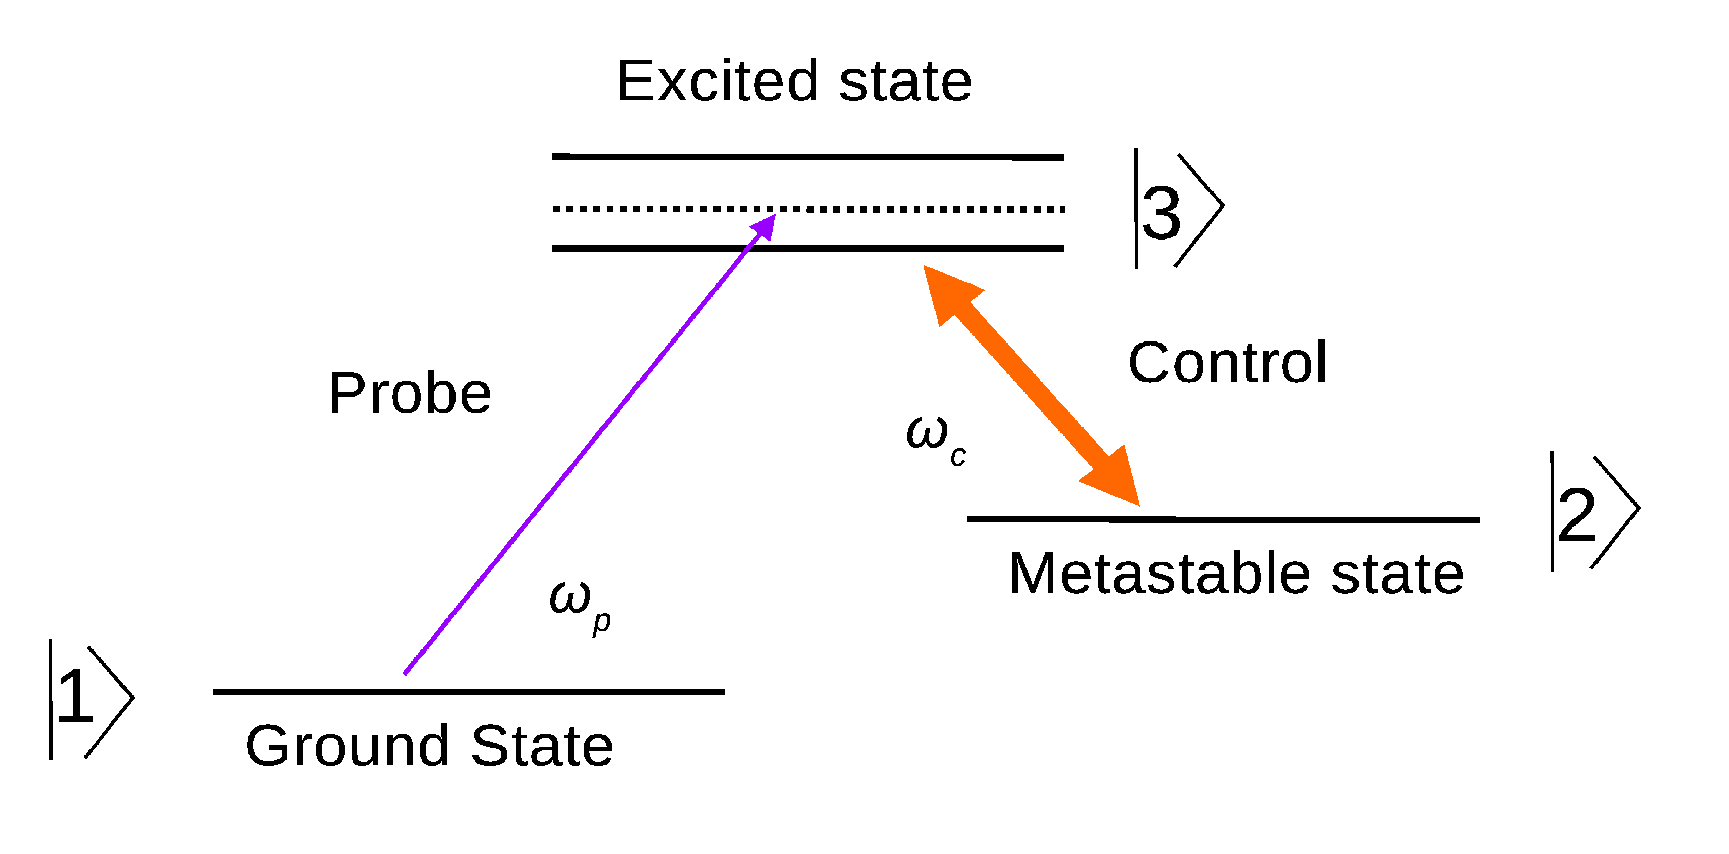
\includegraphics[scale=0.5]{EIT_3_level.eps}
\caption{A three-level atomic system where level three splits due to the presence of much stronger control laser field.}
\end{figure}

\subsection{Three Level Atoms}
To comprehend the occurrence of EIT, we focus on a Lambda-type three-level system shown in Fig. 3.1. In this system, we will discuss what happens quantum-mechanically for the effect of EIT, without disrupting the essence of classical phenomenons. The probability amplitudes of level $\ket{3}$ are driven by two terms in the system. One is the transition probability amplitude of the ground state $\ket{1}$ to the excited state and the other is the oppositely phased transition probability amplitude of the state $\ket{2}$ to the excited state. These both driving fields are opposite in signs but equal in magnitudes and have a frequency $\omega_{p}$ and are so balanced that probability amplitude of state $\ket{3}$ and the expected value of the amplitude of the sinusoidal motion at every frequency that has been applied is zero. 


One may ask how that opposite phase for a transition from the coherent states $\ket{1} \to \ket{2}$ along with the applied field $\omega_{c}$, makes absolute cancellation? Because we use the laser pulses that generate fast enough laser photons that the phase of transitions is maintained and is the correct phase for cancellation [2]. 

 
\section{Coupled Resonator Induced Transparency \\ (CRIT)}
We can observe EIT-like properties in various types of coupled-resonator systems. However, the scope of this thesis is limited to ring resonators systems only. The optical analog of EIT is referred to as Coupled Resonator Induced Transparency (CRIT). This kind of geometry (that we discussed in section 2.4) has been promising for a long time in the field of photonics. EIT analog can be explained based on destructive interference between two electromagnetic fields which circulates the ring resonator system. This system is mostly explained by classical wave travel [3].

\begin{figure}[h]
\centering
\includegraphics[scale=1]{coupled_ring_EIT1.png}
\caption{CRIT in a two ring resonator system.}
\end{figure}


The resonant incident light is coupled to the first ring through the evanescent field and circulates inside the ring and acquires a phase shift of 2$\pi$ after one round trip inside the optical cavity. The circulating light thus interferes constructively with the incoming light and a large intracavity is realized inside the resonator i.e. their phases match perfectly, then at those frequencies, there is a transparency window in the absorption spectrum i.e. a narrow dip, or we see a sharp peak in the transmission spectrum [2].


Figure 3.2 displays the reproduced plot of transmitted intensity vs round-trip phase $\phi$ in a coupled resonator system (as shown in Fig. 2.16 in chapter 2). The parameters used here $r_{1} = 0.9$ and $r_{2} = 0.999$ and attenuations $a_{1} = 0.88$ and $a_{2} = 0.9999$ for first and second resonator respectively. Reproduced from the original work on \textit{``Coupled resonator induced transparency"} [3] from 2004.


Now let us look at the phase response of such a coupled-resonator system. Figure 3.3 shows the effective phase of the entire system (red) and the phase of the transmitted field of the second resonator, in yellow. 

\begin{figure}[h]
\includegraphics[scale=0.75]{coupled_ring_EIT1_phase.png}
\includegraphics[scale=0.75]{coupled_ring_EIT1_coupling.png}
\caption{Effective phase of the system (red) and transmitted phase (yellow) vs round-trip internal phase.}
\end{figure}

Figure 3.4 shows the derivative of the phase of the system which gives us information about the group index and group velocity of the system. 

This value is directly related to the group index of the system. From the graph, we can see that there are negative group-index values for off-resonance regions and positive values on resonances. This informs us that we have superluminal light away from resonance while at resonance subluminal light is produced. 

\begin{equation}
\frac{1}{v_{g}} = \frac{n}{c} \frac{d\phi_{eff}}{d\omega}
\end{equation}

where, group index and group velocity are related by, 
\begin{align*}
n_{g} = \frac{c}{v_{g}}
\end{align*}

\begin{figure}[h]
\centering
\includegraphics[scale=1]{coupled_ring_EIT1_deri.png}
\caption{Derivative of the transmitted phase of the system vs round trip phase.}
\end{figure}

\section{Electromagnetically Induced Absorption}
In contrast to EIT, in Electromagnetically Induced Absorption (EIA), constructive interference occurs between the transition probability amplitudes occurring across two transition pathways. This leads to a narrow dip at the center of the transmission dip in the spectrum of the system, known as Electromagnetically Induced Absorption (EIA) shown in Fig. 3.5. As a whole, EIA is not a very well understood phenomenon and its explanation lacks the true essence.

\begin{figure}[h]
\centering
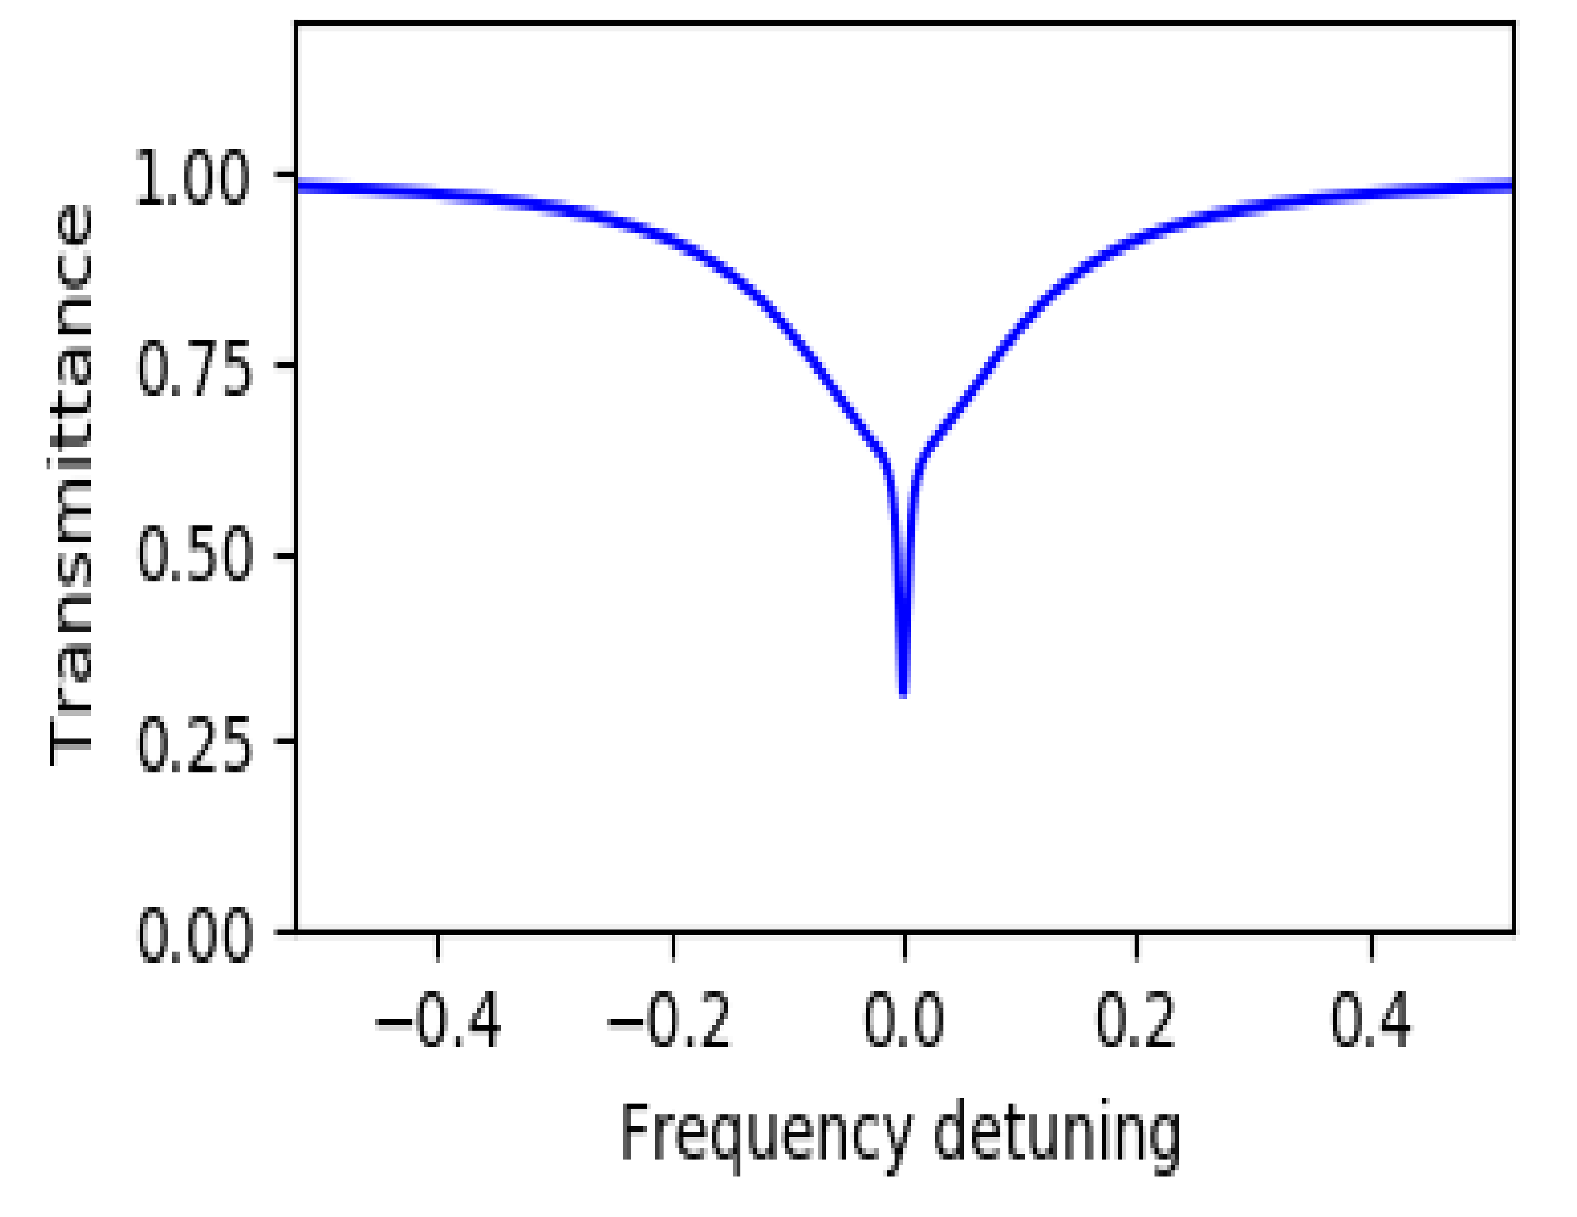
\includegraphics[width=0.5\textwidth]{EIA_basic.eps}
\caption{CRIA in a coupled two ring resonator system.}
\end{figure}

\section{Coupled Resonator Induced Absorption} 
 
Coupled resonator system as discussed above also displays EIA-like effect. The optical analog of EIA is known as Coupled Resonator Induced Absorption (CRIA). CRIA can give us both fast light and slow light, most of the light leading to a different set of broad applications. The system discussed below is again a two-ring resonator system as above and we will again follow the same procedure. Fig. 3.5 displays the CRIA in ring resonator system with coupling parameters as $r_{1} = 0.8998$ and $r_{2} = 0.9998$


\subsection{CRIT in a Passive System}
As before, now we are going to observe what changes does the system has when we introduce gain in it. For convenience, we will first see the passive results for a system and then introduce gain in either in second resonator or first resonator and then introducing gain in both of the resonators. This can be introduced by pumping some monochromatic light source or a laser, in either one of the rings which will drastically compensate the losses inside the resonator and will increase the overall output transmission of the system even above the incident light source. The system parameters are as follows, $r_{1} = 0.9889$ and $r_{2} = 0.9998$ with $Q_{1} = 1\times10^{5}$ and $Q_{2} = 1\times10^{6}$ for first and second resonator respectively (Fig. 3.6). 

\section{Gain-controlled CRIT in coupled resonator}
We observe EIT in a coupled two resonator system, the transmission and effective phase of the system is shown in Fig. 3.6 displaying normal dispersion meaning slow light in the system.

\begin{figure}[h]
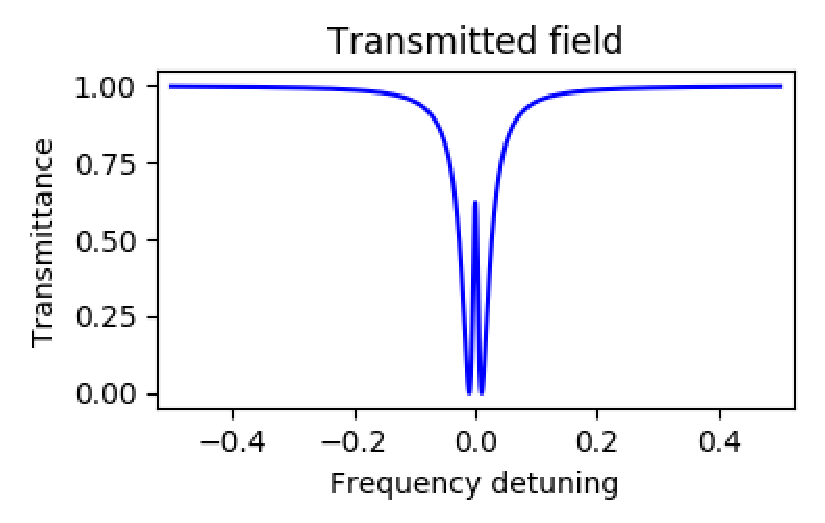
\includegraphics[scale=0.5]{EIT_1.eps}
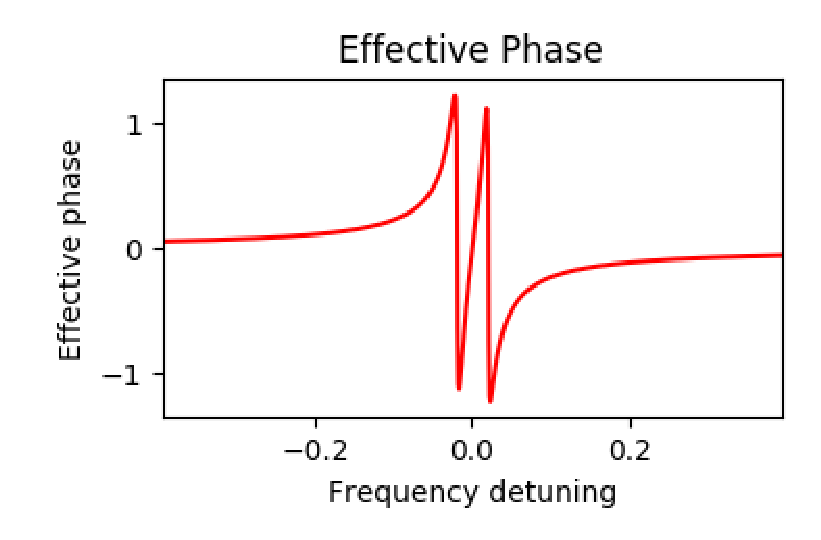
\includegraphics[scale=0.5]{EIT_phase.eps}
\caption{CRIT with its effective phase in a passive resonator system.}
\end{figure}

\subsection{Introducing Gain Only In Second Resonator}
Now we will activate gain in the second resonator, which has higher Q-factor (labeled 2 in Fig. 3.7). We increase the gain to compensate for the intrinsic losses, denoted by $\alpha_{i}$, which is directly related to the Q-factor of the resonator. The transmission peak of the EIT starts to rise gradually to $g$, the gain coefficient is increased. The peak rises towards unity up till $g_{2} \to \alpha_{i,2}$, where alpha is the attenuation constant for intrinsic loss. 

\begin{figure}[h]
\centering
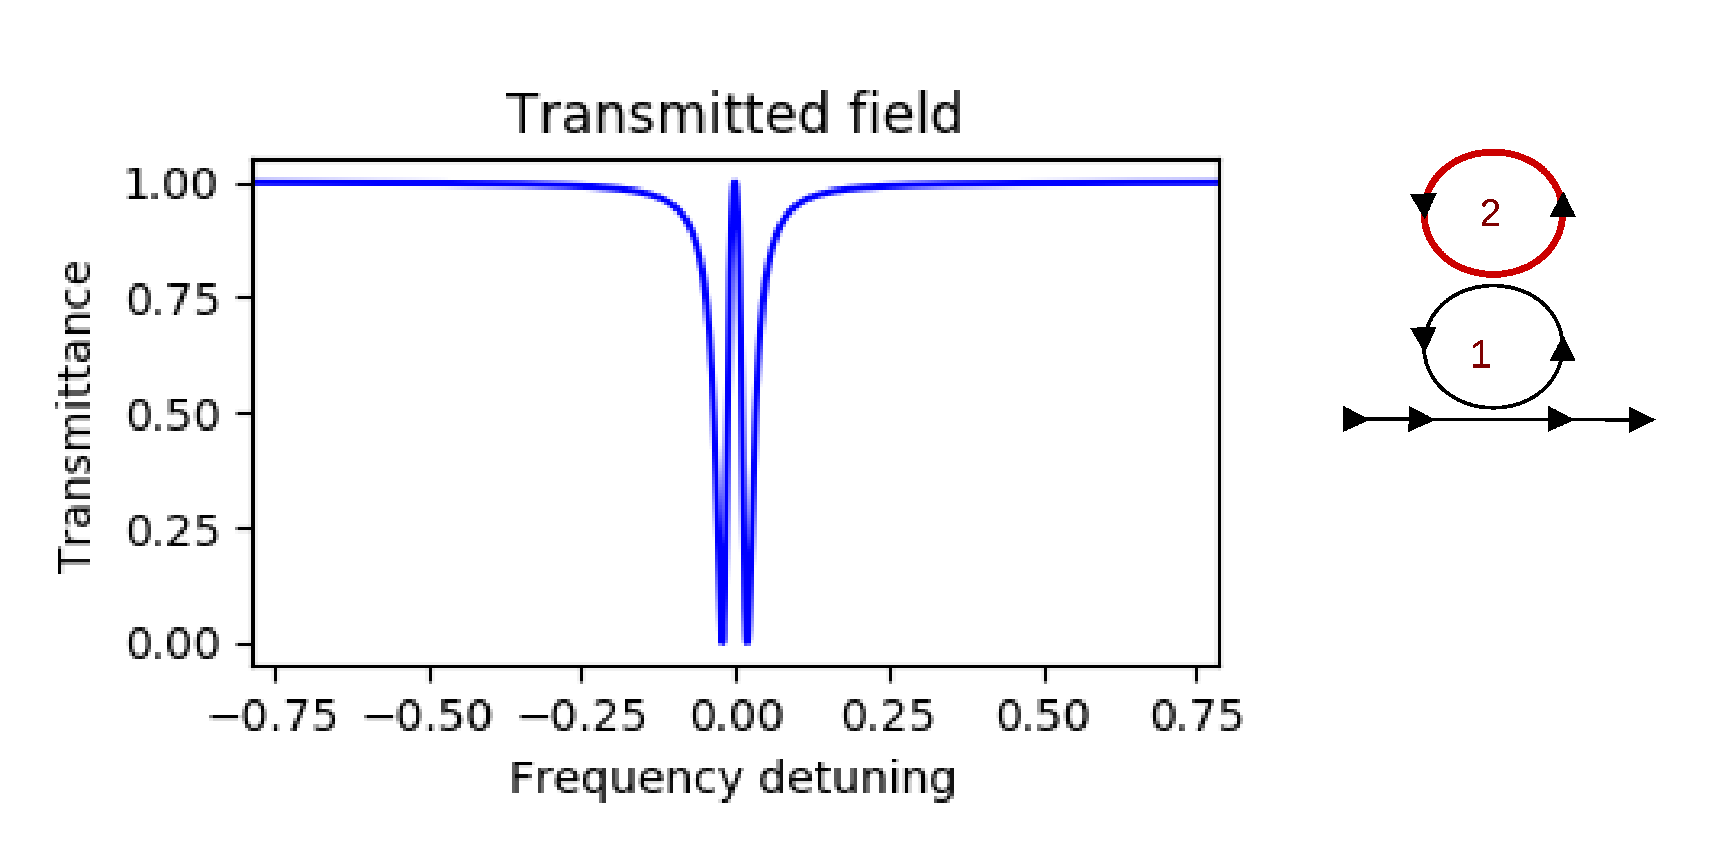
\includegraphics[scale=0.5]{EIT_gain2.eps}
\caption{CRIT in an active coupled resonator system.}
\end{figure}

When gain coefficient equals the intrinsic loss coefficient, i.e. $g = \alpha_{i}$, the peak of the transmission touches the unity on the graph this implies that all of the incident light is verily being transmitted the other side i.e. the medium has become completely transparent for resonant frequencies. This means that we have now compensated for all the losses inside the system which are intrinsic. When this happens, we see an abrupt change in the effective phase of the system. This system now gives us anomalous dispersion on-resonance meaning we get fast light in EIT (Fig. 3.8). 

To get a brief idea of what is happening, I have also calculated the group index of the system. In this case, we receive negative values for the group index $n_{g}$ on resonance. Fig. 3.9 displays the group index for this particular case.


\begin{figure}[h]
\centering
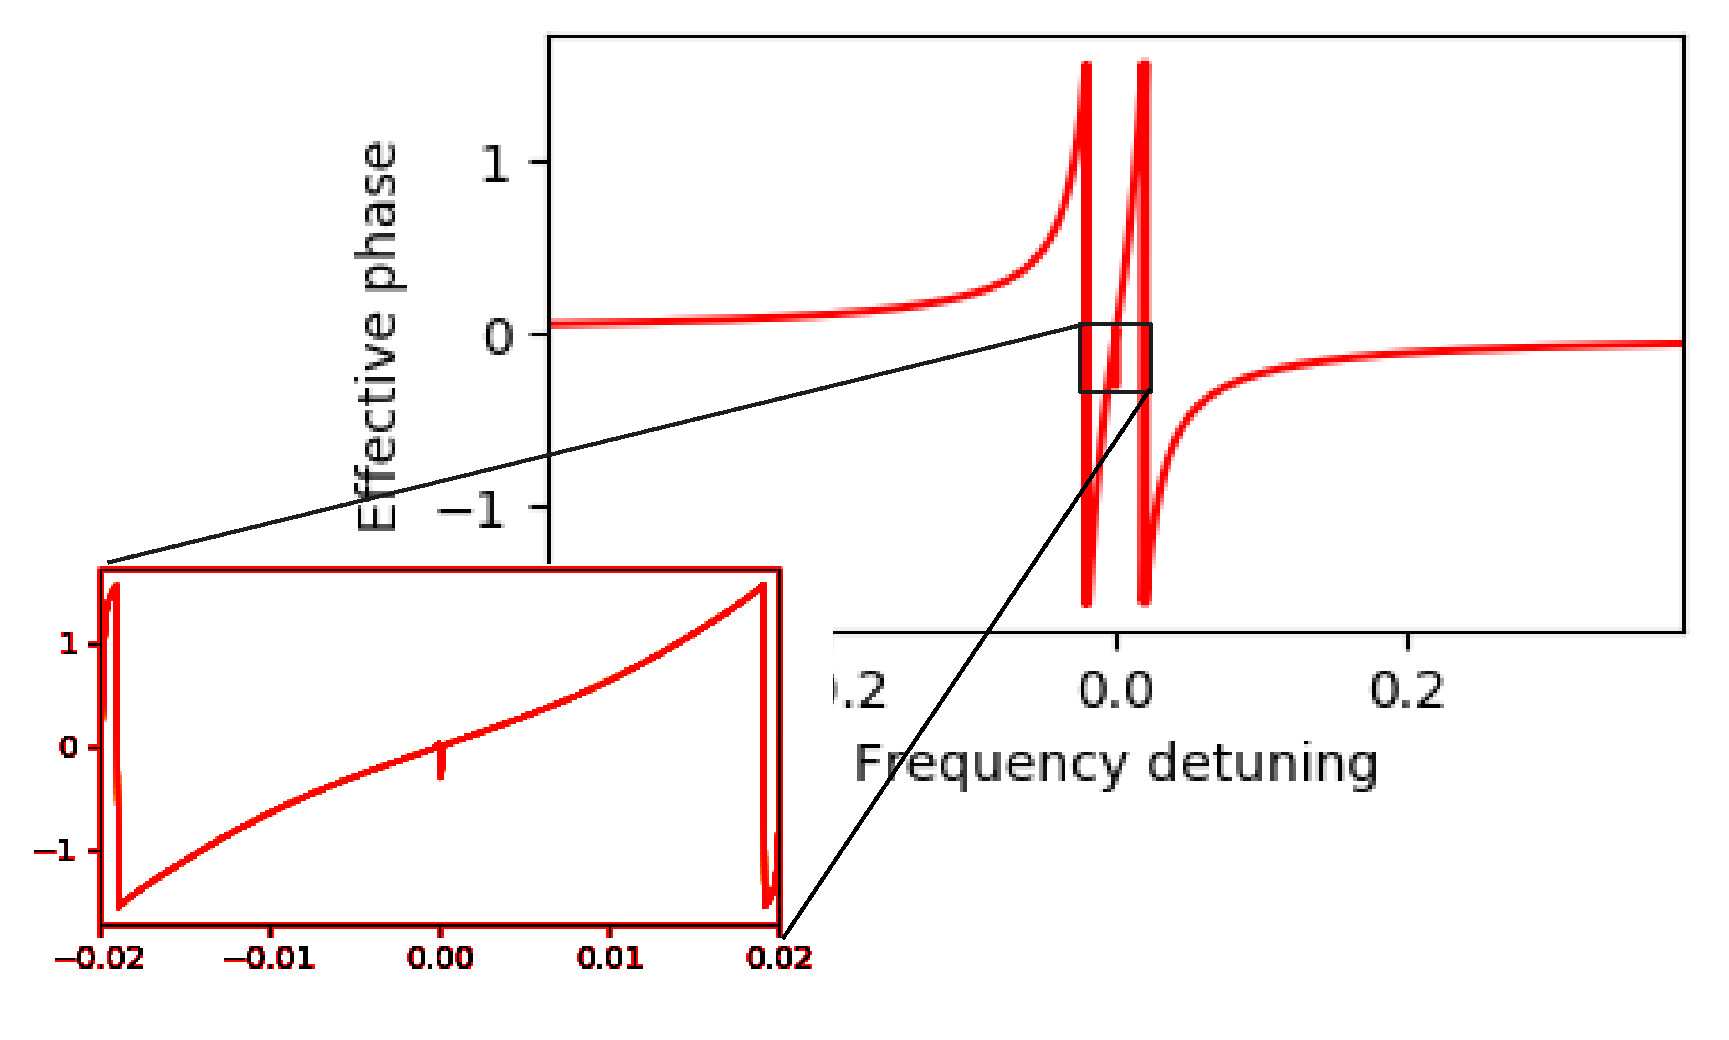
\includegraphics[scale=0.30]{EIT_gain2_phase.eps}
\caption{Effective phase of CRIT in an active coupled resonator system. Magnified view of phase near resonance frequency is shown.}
\end{figure}

     
\begin{figure}[h]
\centering
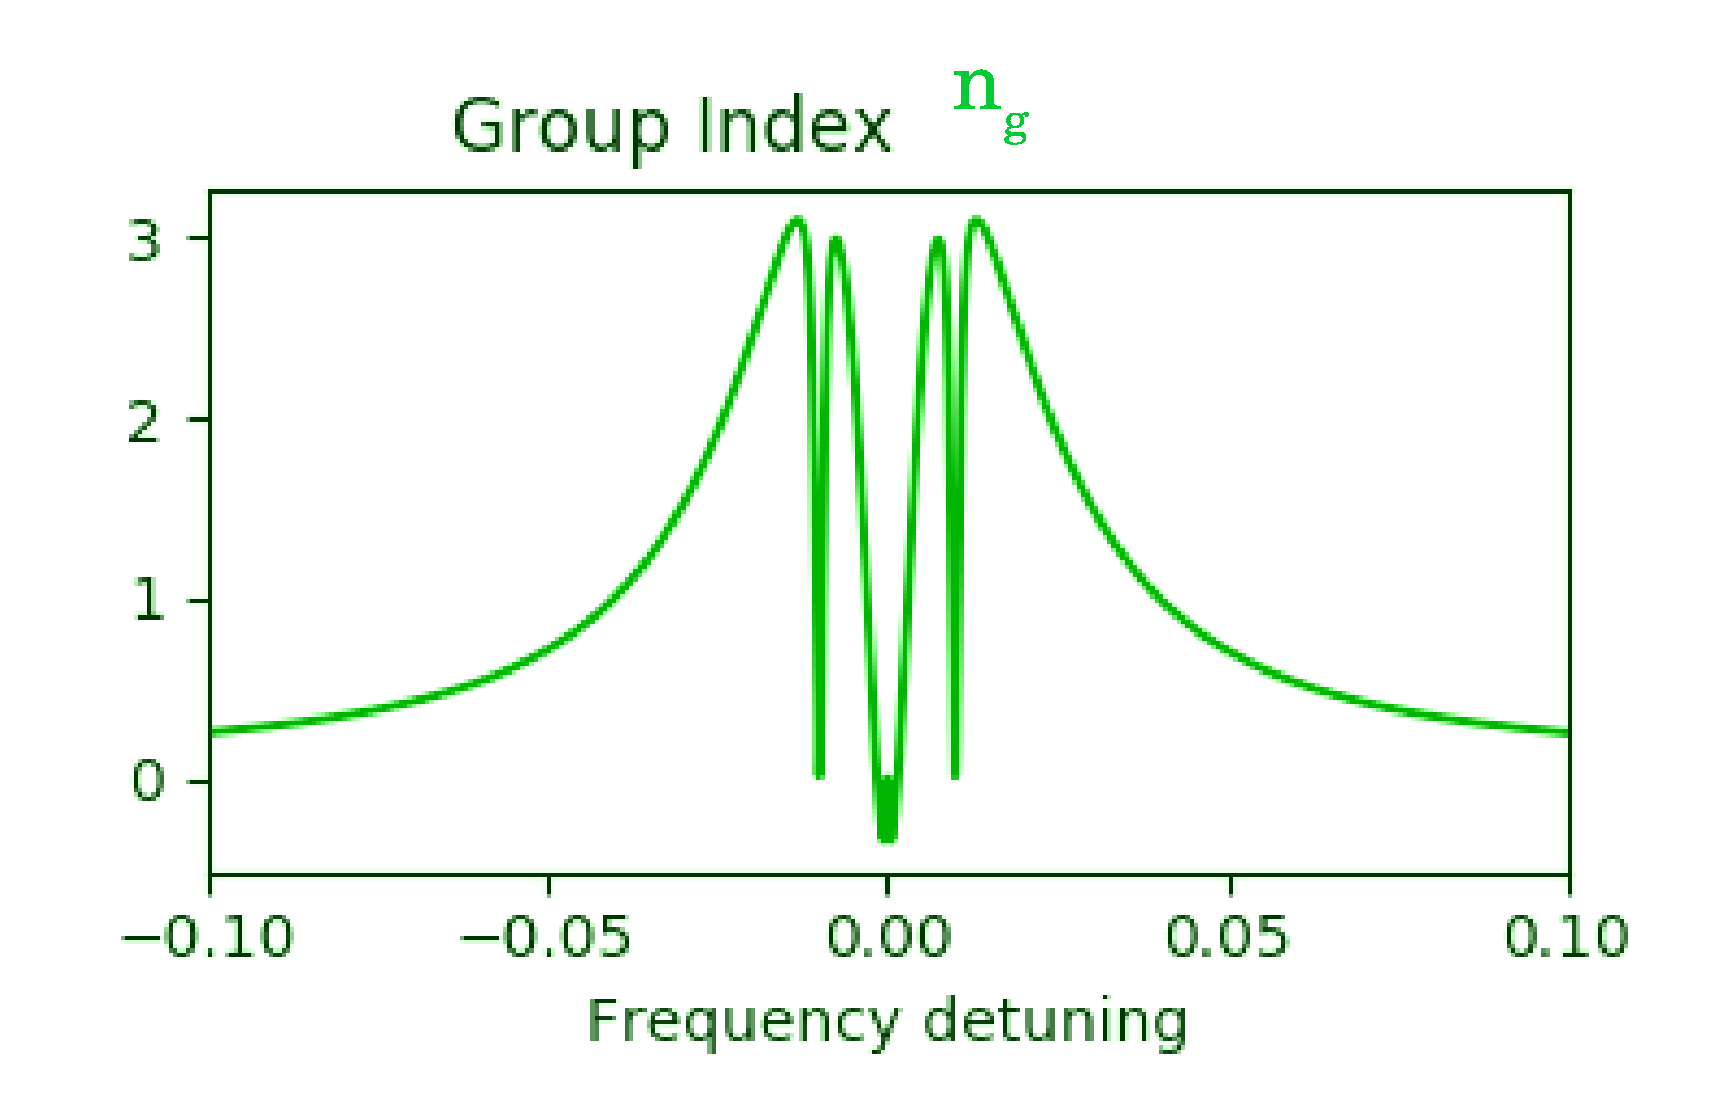
\includegraphics[scale=0.30]{EIT_gain2_ng.eps}
\caption{Group index of an active resonator system showing negative values on resonant frequency.}
\end{figure}


\subsection{Introducing Gain Only In First Resonator}
Now we will activate gain in the first resonator (labeled 1), which has lower Q-factor in comparison to the second resonator. The spectrum of the EIT starts to rise and displays a hanging EIT. (Fig. 3.10)

\begin{figure}[h]
\centering
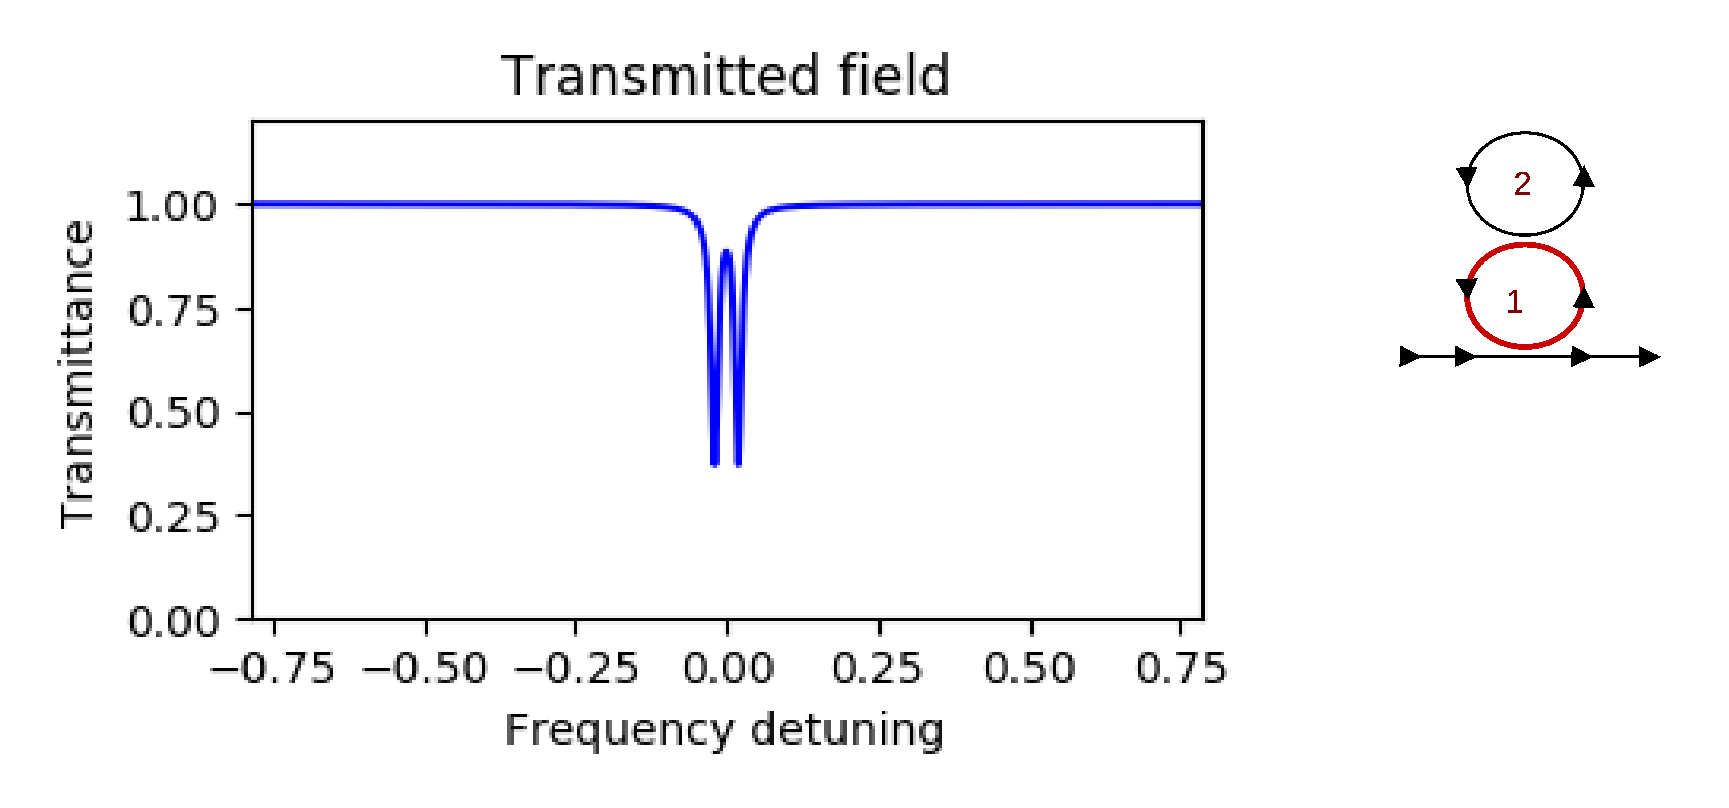
\includegraphics[scale=0.35]{EIT_gain1.eps}
\caption{CRIT of the two resonator system with gain activated in resonantor 1.}
\end{figure}

The effective phase of the system remains similar to a passive resonator, displaying normal dispersion (slow light). The index value on resonance calculated to be about $\approx 76.2$ which shows that light has been slowed down only marginally for this case (Fig. 3.11). 

\begin{figure}[h]
\includegraphics[scale=0.5]{EIT_gain1_phase.png}
\includegraphics[scale=0.5]{EIT_gain1_ng.png}
\caption{Effective phase shows normal dispersion (in red) and group index $n_{g}$ shown in green.}
\end{figure}


\subsection{Introducing Gain In Both Resonators}
Now we will activate gain in both of the resonators simultaneously such that the ratio of the gain coefficients, $g_{1}$ and $g_{2}$, are the same. We observe that the peak of the EIT, as well as the whole transmission, starts to rise towards unity as $g_{1,2} \to \alpha_{i}$ (Fig. 3.12). The EIT transmission window also narrows down gradually.

\begin{figure}[h]
\centering
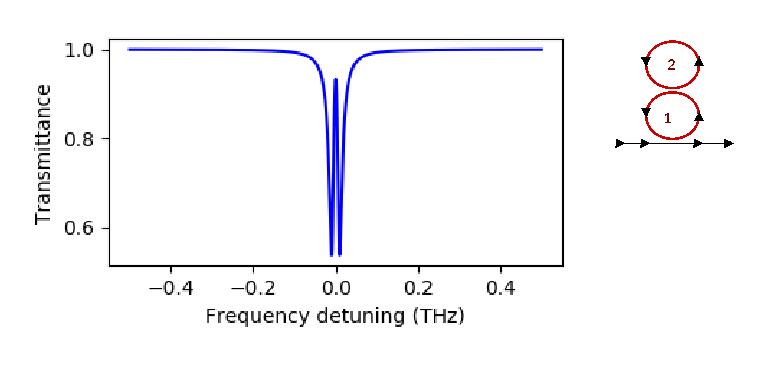
\includegraphics[scale=0.70]{EIT_gain12.eps}
\caption{Transmission graph of two resonator system with gain activated in both.}
\end{figure}

The effective phase of the system shows rather distinct curves which are basically due to the artifacts in the system or computation errors. The on-resonance information tells us that we have normal dispersion and positive group index about $\approx 766.5$ (Fig. 3.13). 

\begin{figure}[h]
\centering
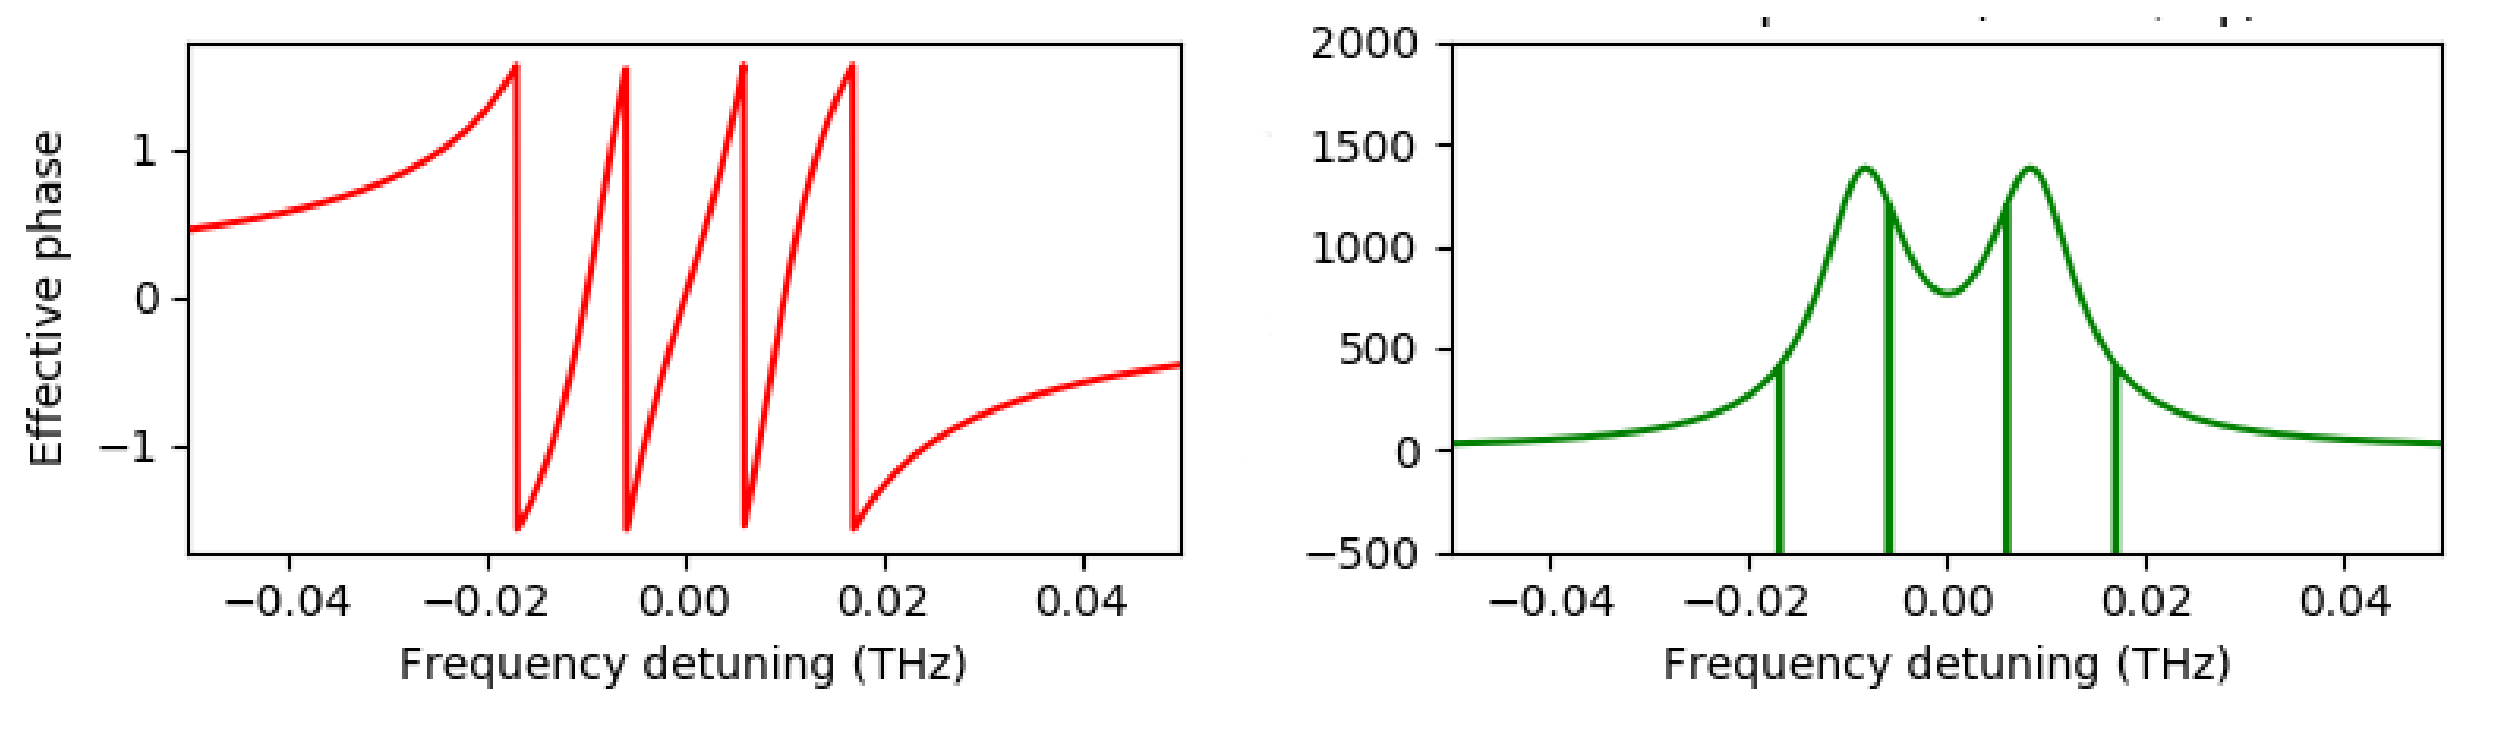
\includegraphics[scale=0.35]{EIT_gain12_phase.eps}
\caption{Phase and group index of a resonator system with gain in both resonators.}
\end{figure}

When the gain coefficient $g$ becomes greater than the intrinsic loss coefficient $\alpha_{i}$, then the whole transmission graph flips about the horizontal axis and we now see a distinct spectrum with a reversed EIT shown in Fig. 3.14.

\begin{figure}[h]
\centering
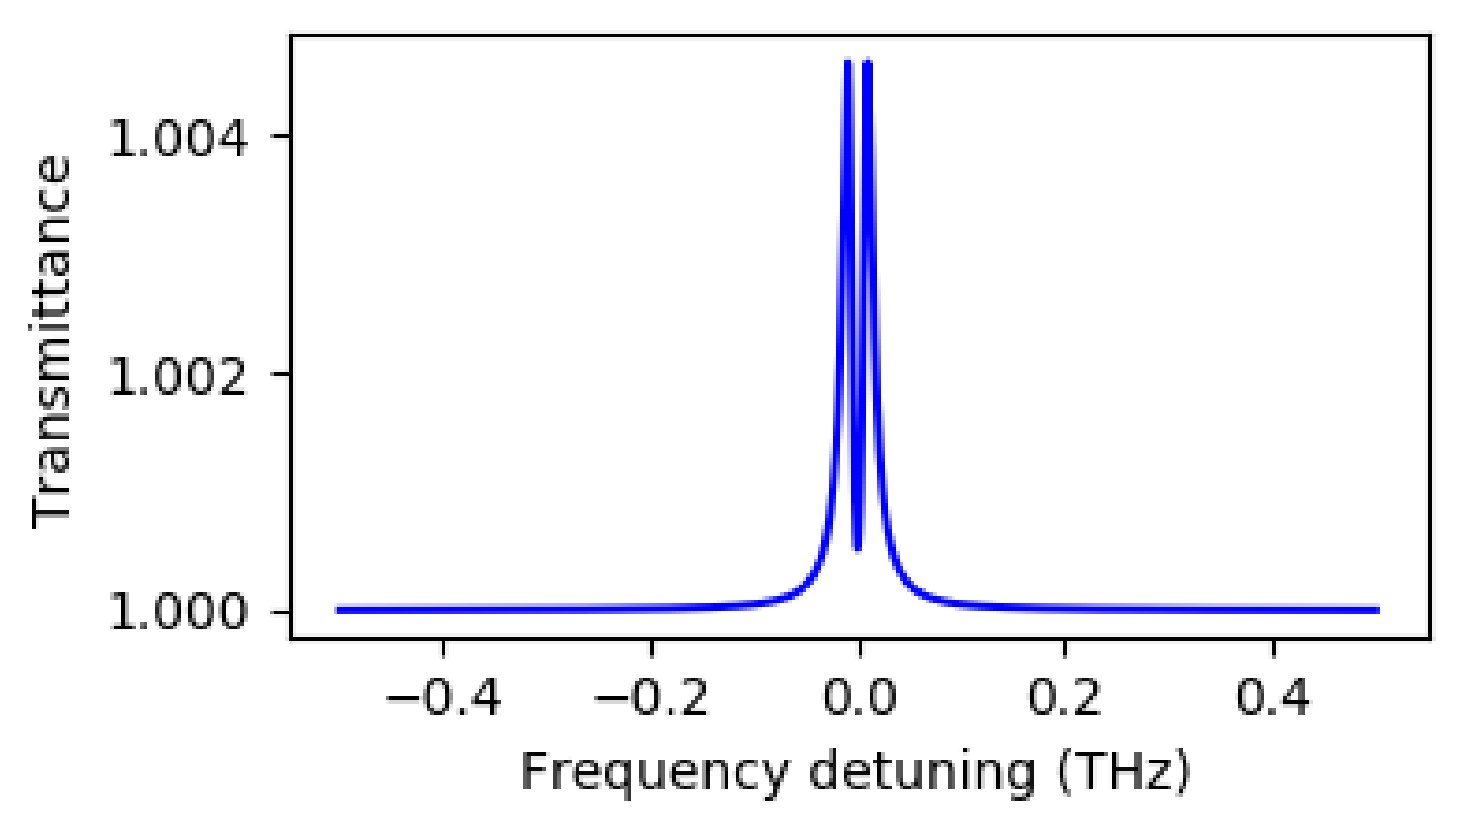
\includegraphics[scale=0.35]{EIT_gain12b.eps}
\caption{Flipping of the EIT spectrum when gain coefficient is larger than the attenuation coefficient.}
\end{figure}

This flipping of the transmission does not affect the dispersion of the medium. This means the effective phase and the group index of the system are similar in this case. However, we now have a transmission peak which is above unity. This shows that due to gain, intrinsic losses have been compensated and a transparent coupled resonator system is achieved.


  

\section{Gain-controlled CRIA in Coupled Resonators}
Now we will observe the behavior of the transmission spectrum of CRIA when we introduce gain in it. Similarly, first we are going to activate again in the second resonator, then into the first resonator and in last we activate and increase gain in both resonators simultaneously. 

\subsection{CRIA With Slow Light in Passive Coupled Resonators}
We will first examine the response of the CRIA (Fig. 3.5) in a passive medium with having normal dispersion. shown in Fig. 3.15, with its group index.

\begin{figure}[h]
\centering
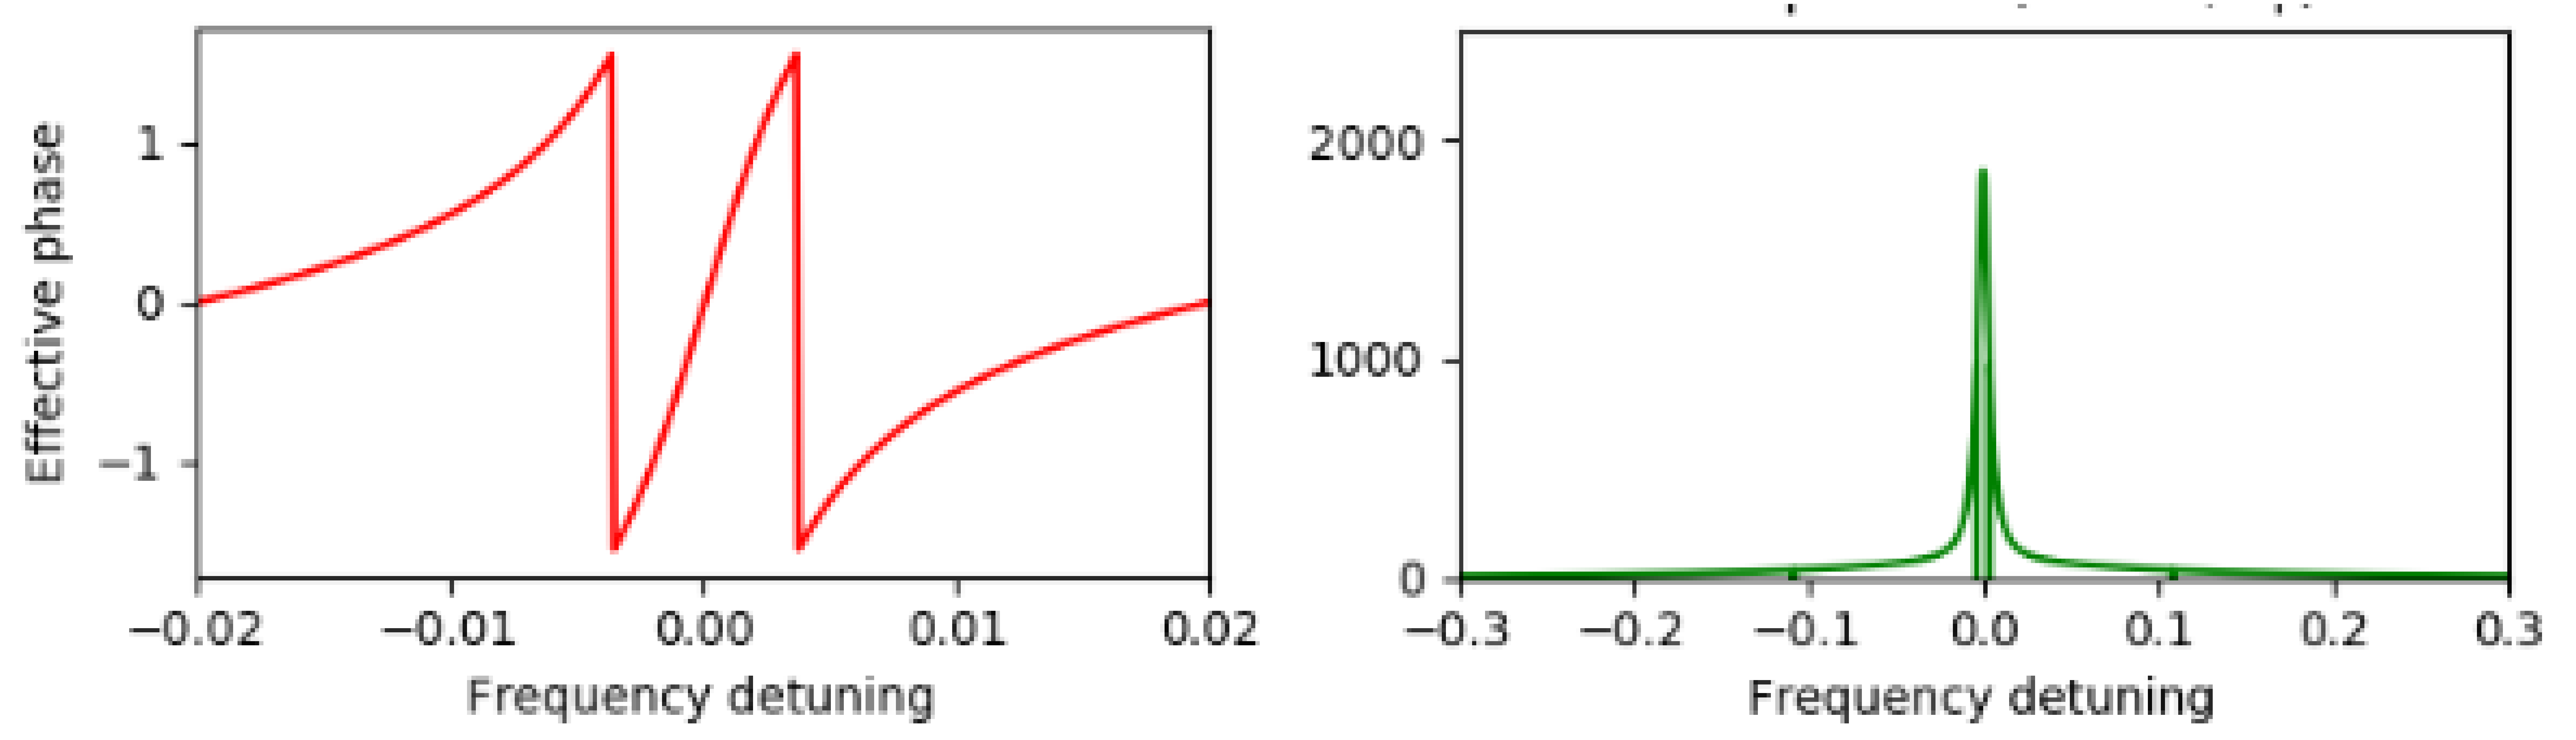
\includegraphics[width=1\textwidth]{EIA_gain_phase1.eps}
\caption{Phase and group index of CRIA.}
\end{figure}
  
\subsection{Introducing Gain Only In Second Resonator}
Now we activate gain in the second resonator such that $g \leqslant \alpha_{i}$.  When the gain becomes closer to the value of $\alpha_{i}$ ($g \to \alpha_{i}$), the EIA spectrum changes into EIT type transmission (Fig. 3.16).

\begin{figure}[h]
\centering
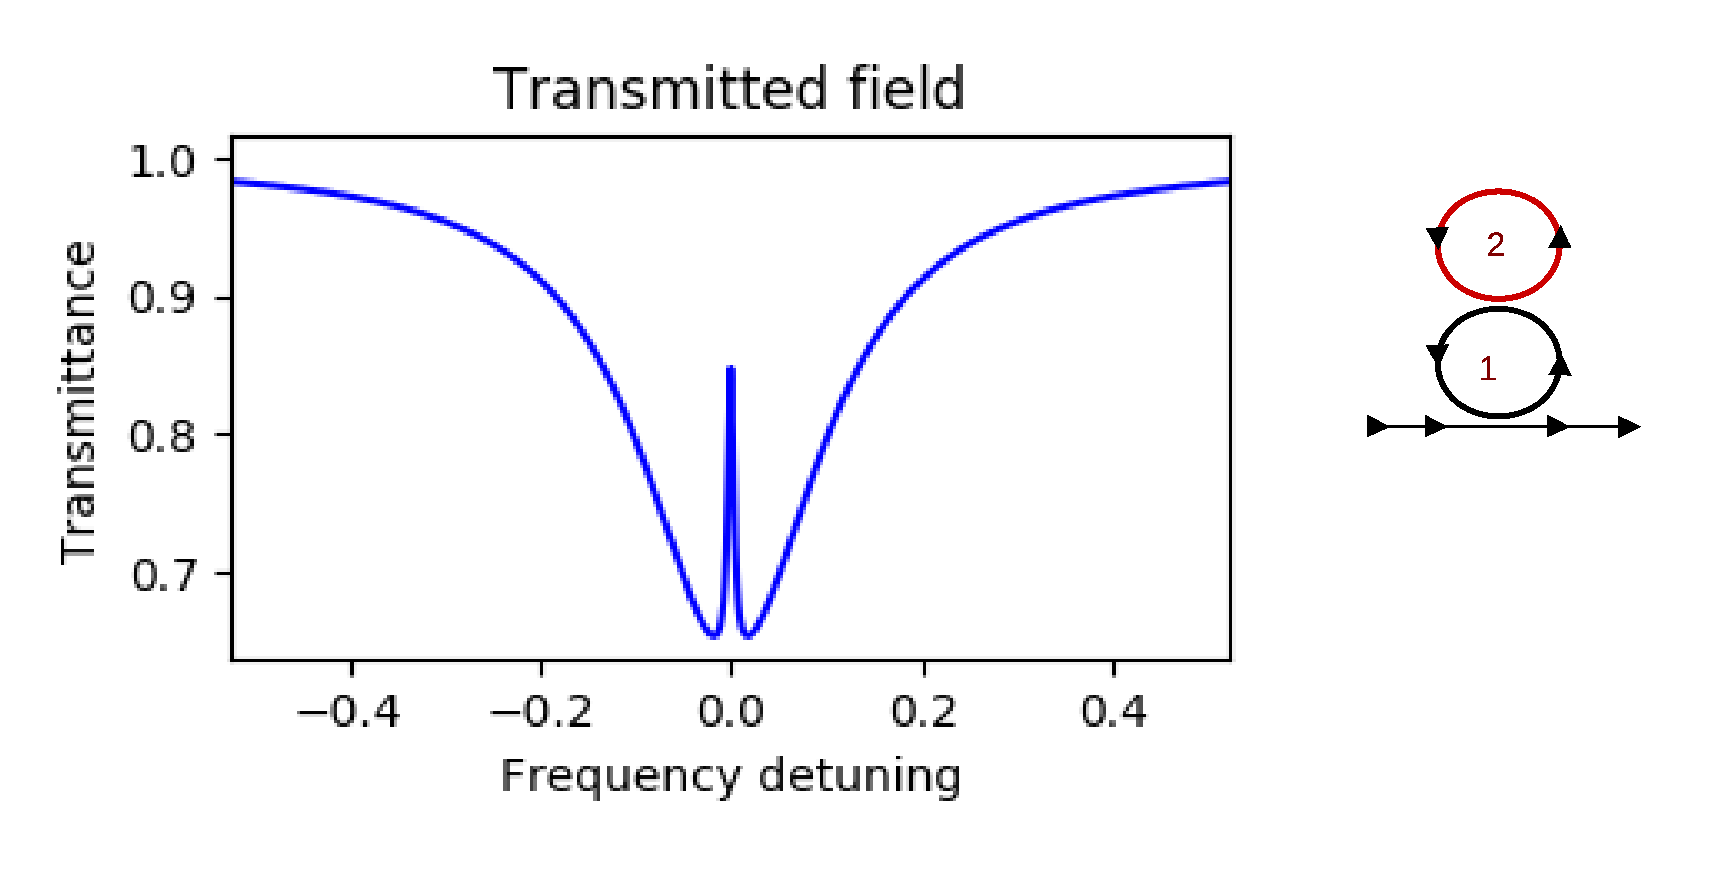
\includegraphics[scale=0.30]{EIA_to_EIT.eps}
\caption{CRIA dip changes from Fig. 3.5 into an CRIT type transmission when gain is introduced in second resonator.}
\end{figure}

The effective transmission phase changes from normal dispersion to anomalous dispersion. Corresponding group index displays a negative value of $n_{g} \approx -4505$ at resonance, implying a negative group delay and therefore, superluminal light (Fig. 3.17). Thus EIT which, in a passive coupled resonator system, always yields slow light, now enables superluminal (fast light) group velocities of resonant frequencies.

\begin{figure}[h]
\centering
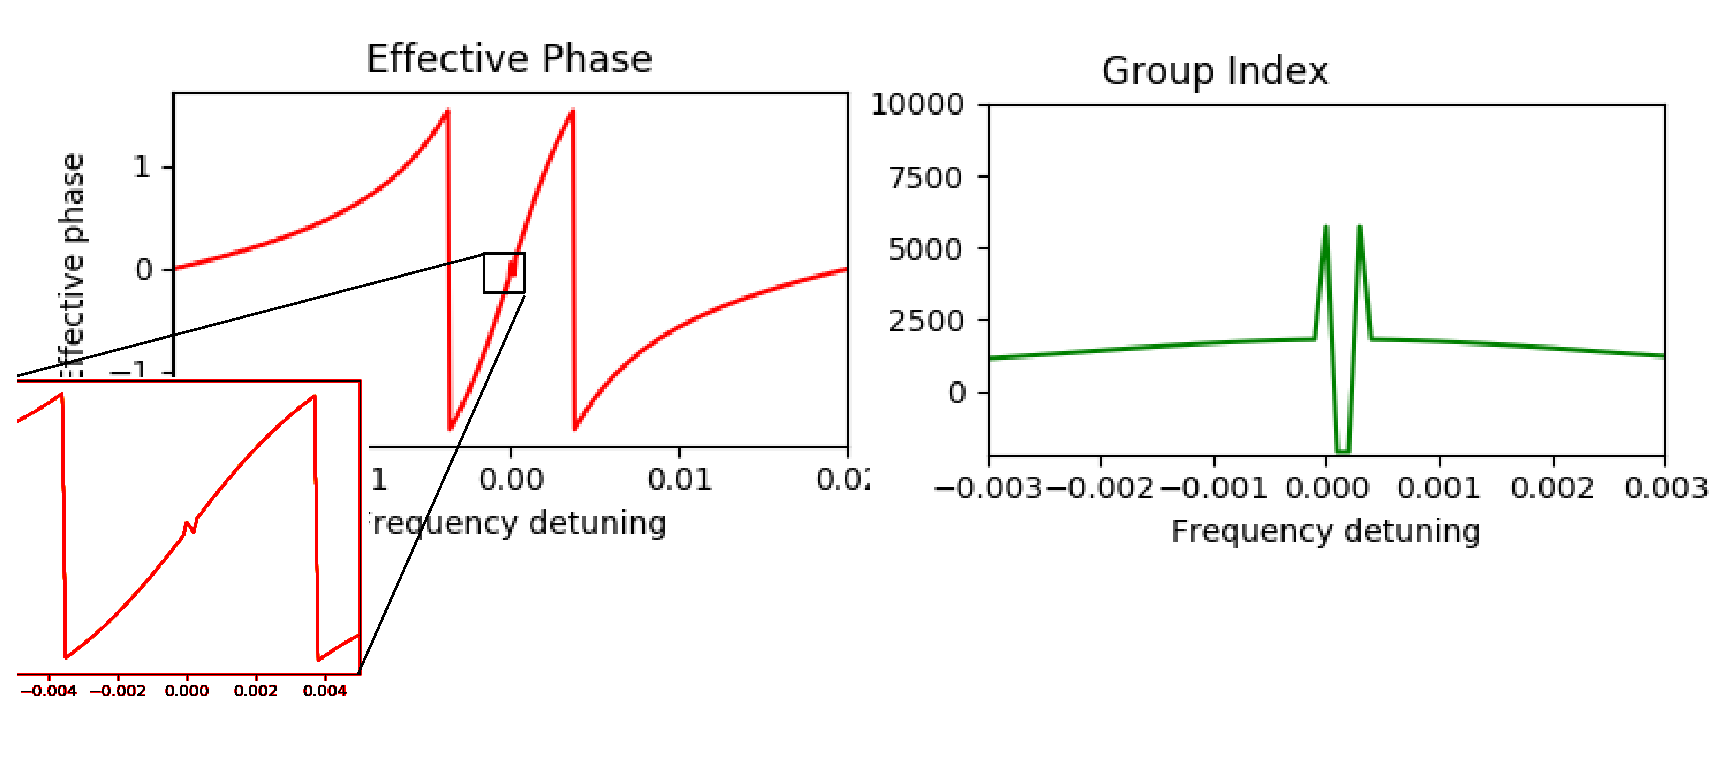
\includegraphics[scale=0.45]{EIA_to_EIT_phase.eps}
\caption{Phase of the system showing anomalous dispersion on resonance (zoomed) and group index showing negative values.}
\end{figure}

\subsection{Introducing Gain Only In First Resonator}
Now we activate gain in the first resonator (labeled 1 in Fig. 3.18) and observes that the EIA resonance narrows down and eventually becomes a sharp transmission dip. Fig. 3.18. Corresponding transmission phase and group index reveal normal dispersion and slow light (Fig. 3.19).


\begin{figure}[h]
\centering
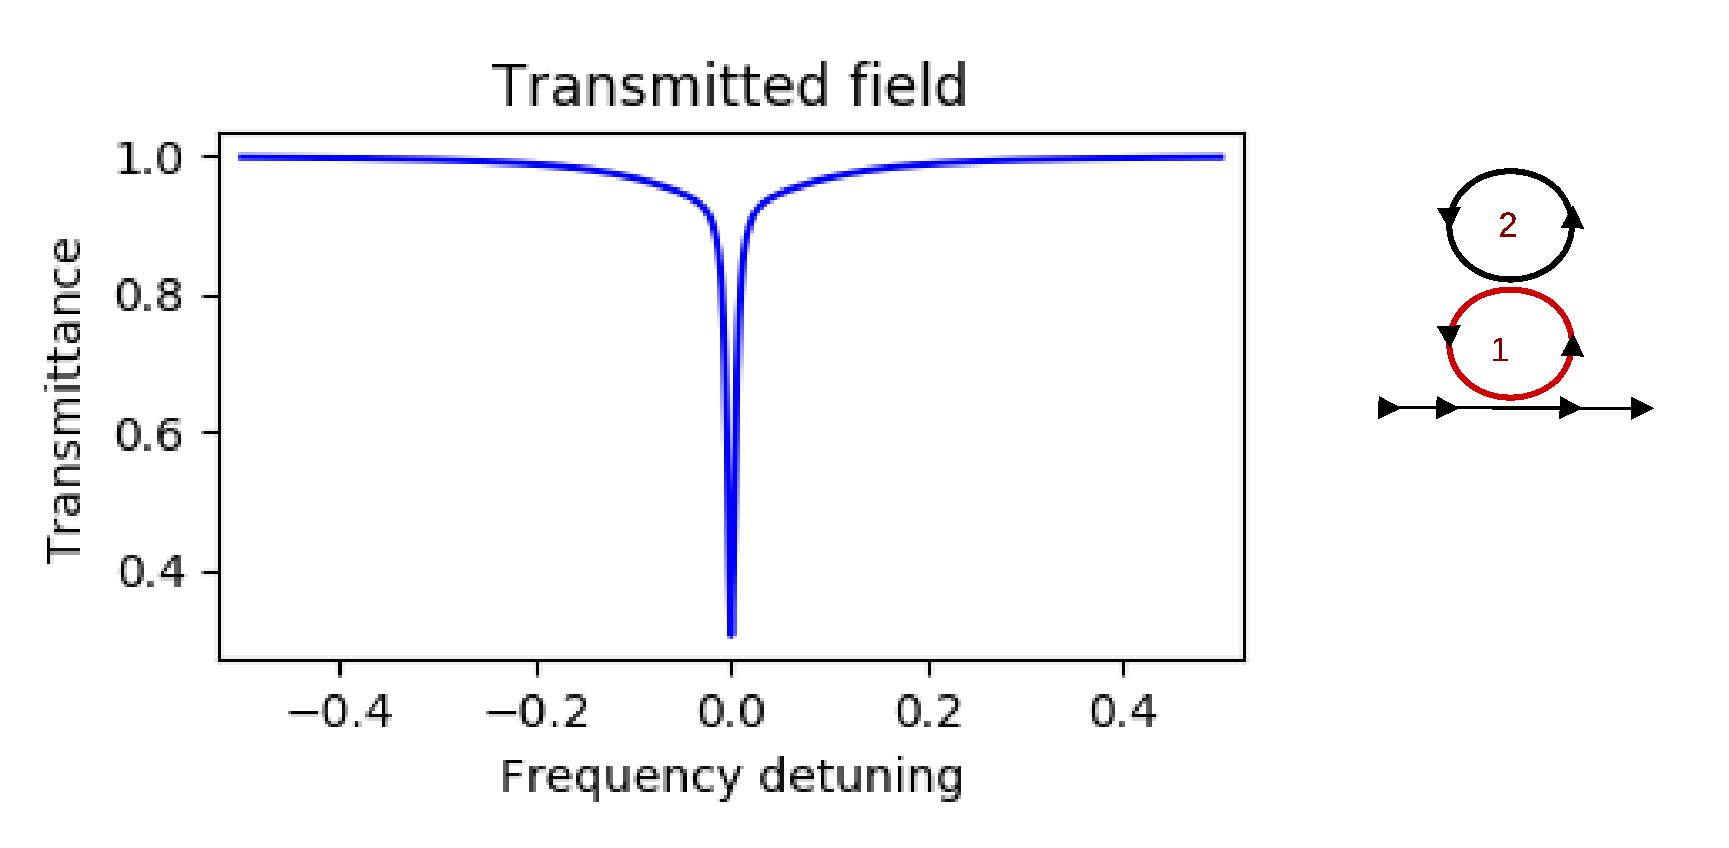
\includegraphics[scale=0.30]{EIA_gain1.eps}
\caption{CRIA with gain activated in first resonator.}
\end{figure}

\begin{figure}[h]
\centering
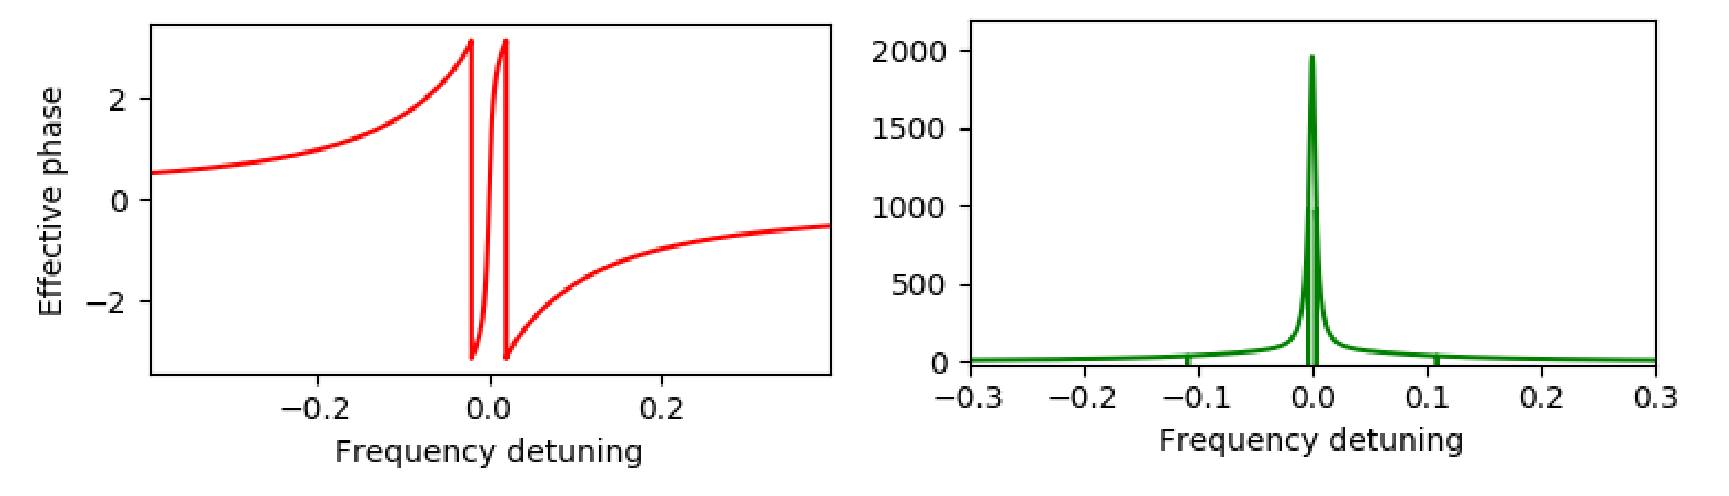
\includegraphics[scale=0.45]{EIA_gain1_phase.eps}
\caption{CRIA phase and group index.}
\end{figure}


\subsection{Introducing Gain In Both Resonators}
Now we consider the case where the gain is activated in both of the resonators simultaneously. No notable changes occurs in the transmission spectrum when $g_{1}$ and $g_{2} < \alpha_{i}$. Fig. 3.20. The phase and group index is also shown in Fig. 3.21.

\begin{figure}[h]
\centering
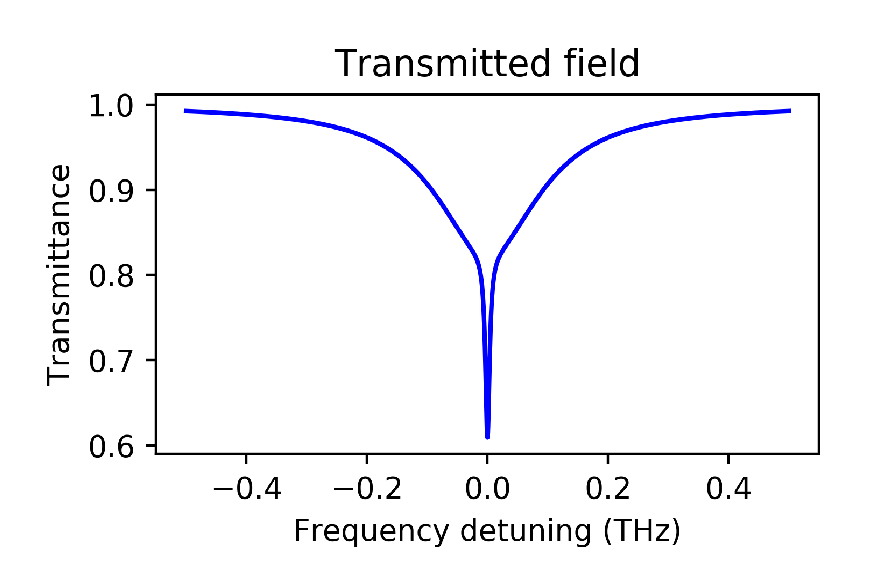
\includegraphics[scale=0.45]{EIA_gain12.eps}
\caption{CRIA with gain in both resonators.}
\end{figure}


\begin{figure}[h]
\centering
\includegraphics[scale=0.5]{EIA_gain12_phase.eps}
\caption{CRIA phase in red and group index in green.}
\end{figure}

However, if gain becomes closer to intrinsic loss, i.e. $g \to \alpha_{i}$, the transmission spectrum values are very near to 1 now and we see anomalous dispersion in the effective phase of the system and negative group index of about $\approx -4550$ (see Fig.3.22).

\begin{figure}[h]
\centering
\includegraphics[scale=0.5]{EIA_gain12b.eps}
\includegraphics[scale=0.45]{EIA_to_EIT_phase.eps}
\caption{Transmission rises towards unity, dispersion becomes anamolous on resonance, and group index displays negative values.}
\end{figure}

With further increase in the gain, the spectrum flips over the horizontal axis and EIA turns into an EIT like transmission Fig. 3.23. The dispersion remains anomalous as the gain is further increased, i.e. $g > \alpha_{i}$. After the gain achieves a threshold value, again a transition occurs and anomalous dispersion is converted into normal dispersion (Fig. 3.24).

\begin{figure}[h]
\centering
\includegraphics[width=0.40\textwidth]{EIA_gain12ab.eps}
\caption{Transmission of the system}
\end{figure}

\begin{figure}[h]
\centering
\includegraphics[width=1\textwidth]{EIA_gain_phase1.eps}
\caption{Phase and group index of the system.}
\end{figure}

It is worth noting that the EIT-like resonance shown in Fig. 3.23, usually gives slow light in passive resonators [8]. However, in the present case, fast light is obtained owing to the incorporation of a gain element into the system until a specific threshold gain value.

\subsection{CRIA With Fast Light in Passive Coupled Resonator}
Now we will consider a case featuring CRIA which leads to fast light in a passive coupled resonator system and studies the behavior when the gain is introduced in either one of the resonators. The coupling parameters are given as, $r_{1} = 0.8998$ and $r_{2} = 0.99998$ while the quality factors remains the same. (Fig. 3.25)

\begin{figure}[h]
\centering
\includegraphics[scale=0.65]{EIAf_passive.eps}
\includegraphics[scale=0.5]{EIAf_passive_phase.eps}
\caption{CRIA observed in a passive two resonator system with anamolous dispersion and negative group index.}
\end{figure}

\subsection{Introducing Gain Only In Second Resonator}
Now we activate gain in the second resonator, shown in the schematic (Fig. 3.26), and observes that the EIA resonance narrows down and becomes sharp. While the amplitude of the narrow CRIA feature decreases, resulting in higher transmission. 

\begin{figure}[h]
\centering 
\includegraphics[scale=0.65]{EIAf_gain2.eps}
\caption{Transmission spectrum of CRIA with gain in second resonator.}
\end{figure}


\begin{figure}[h]
\centering
\includegraphics[scale=0.45]{EIAf_gain2_phase.eps}
\caption{Transition from fast to slow light in CRIA.}
\end{figure}

The dispersion of the system changes as gain becomes close to intrinsic loss ($g \approx \alpha_{i}$) and normal dispersion and a positive group index are obtained (Fig. 3.27).

However, when the gain is further increased and it exceeds the intrinsic losses, such that $g > \alpha_{i}$, the spectrum then shows a conversion from CRIA into CRIT (Fig. 3.28) with normal dispersion and positive group index.

\begin{figure}[h]
\centering
\includegraphics[scale=0.60]{EIAf_gain2a.eps}
\caption{Transmission dip transforming into an tranmission peak.}
\end{figure}

However, the dispersion of the system remains unaffected. It is worth noting that although the dispersion remains subluminal for higher transmission, the transmitted light becomes transparent due to CRIT resonance.

\subsection{Introducing Gain Only In First Resonator}
We again start with the passive CRIA of Fig 3.25. However, now we introduce gain in the first resonator only. We observe the CRIA resonance narrows down and becomes a sharp dip. Also, two off-resonance peaks appear in the spectrum. As $g \approx \alpha_{i}$, the resonance becomes further narrower and the system moves towards critical coupling. We still see fast light and negative group index from here but most of the light is absorbed. The transmission spectrum in Fig. 3.29 is shown for $g > \alpha_{i}$.

\begin{figure}[h]
\centering
\includegraphics[scale=0.60]{EIAf_gain1.eps}
\caption{Transmission dip of CRIA with gain in first resonator.}
\end{figure}

\subsection{Introducing Gain In Both Resonator}
If we introduce gain in both of the resonators of an initially passive system (Fig. 3.25), simultaneously, we observe the narrowing of CRIA dip and rise of the transmission towards unity. However, the transmission dip changes into a peak when the gain is greater than intrinsic losses ($g > \alpha_{i}$) owing to the transparency of the system (Fig. 3.30). The CRIT resonance of this transparent system leads to normal dispersion and positive group index of $\approx 2\times10^{4}$ (Fig.3.31).

\begin{figure}[h]
\centering
\includegraphics[scale=0.60]{EIAf_gain12.eps}
\caption{Transmission dip transforming into a tranmission peak.}
\end{figure}

\begin{figure}[h]
\centering
\includegraphics[scale=0.60]{EIAf_gain2_phase.eps}
\caption{Respective phase and group index of the system.}
\end{figure}

These observations lead to the conclusion that when we introduce gain into the system, with it being activated in either one of the resonators or both, we observe drastic changes in the transmission and phase spectrums thus affecting the group delay and dispersion of the system. This allowed achieving gain-assisted tunability of the dispersion of the system, meaning the transitions between fast and slow light can be controlled by simply introducing gain into a passive coupled resonator system.


\section{Proposed Applications}
\subsection{Gain-controlled Optical Pulse Storage and On-demand Retrieval}
Coupling parameter between the two resonators $r_{2}$ can induce very distinct changes into the system.

\begin{figure}[h]
\centering 
\includegraphics[width=0.5\textwidth]{photon_storage.png}
\caption{Single resonance displayed in a coupled resonator system with its transmission phase.}
\end{figure}

Now we will discuss a case in which the coupling between the two resonators is very weak and the resonance of the second resonator is almost zero. Meaning we have a single resonance transmission at critically coupled i.e. all of the light is absorbed. Fig. 3.32 displays the transmission spectrum along with its effective phase displaying anomalous dispersion. 

Now we will excite gain in the second resonator such that the gain coefficient $g_{2}$, is equal to the intrinsic loss coefficient $\alpha_{i}$. In this state, an input optical pulse whose bandwidth matches the CRIT peak can be coupled to the system. This process happens at nanoseconds scale meaning we can switch from zero to maximum intensity in nanoscale durations. Fig. 3.33 displays the gain excited transmission with normal dispersion meaning we have slow light which was the main ambition.

This shows that the light pulse is now stored inside the coupled resonator system and to retrieve the stored pulse back. As soon as the light pulse has entered the system, the gain is turned off. Once again a critically coupled transmission resonance appears in the spectrum. The true shape of the input signal is not disturbed the narrow peak of EIT shows us that very narrow bandwidth of frequencies can be stored. For this case, a narrow bandwidth pulse can be stored in a coupled-resonator. However, by using a lower-Q second resonator a larger bandwidth pulse can be stored.

\begin{figure}[h]
\centering 
\includegraphics[width=0.50\textwidth]{photon_storage_gain.png}
\caption{EIT peak emerges when gain is excited in second resonator in a coupled resonator system. The corresponding transmission phase is also shown.}
\end{figure}

\subsection{Gain Controlled Slow and Fast Light Tuning}
We have observed from these results that the transitions from super and subluminal velocities of light have been in the control of the optical gain of the system. We have observed superluminal regimes of transmission reverting into subluminal transmission by the excitation of gain in either one or both coupled two resonator system. Also, the subluminal transmissions such as EIT which always displays slow light in passive systems provided us with fast light and anomalous dispersion in the presence of gain in either of the resonators. This tuning of gain made possible the transitions between fast and slow light in both ways, meaning we have achieved control over how and when do we want fast and slow light for our device.

\newpage
\section{Discussion}
We showed tunability of optical analogs of Electromagnetically Induced Transparency (EIT) and Electromagnetically Induced Absorption (EIA). This enabled pulses that propagate through system owing to controlled excitation of the gain medium. superluminal and subluminal group velocities of light in a coupled ring resonator framework, with a direct increase excitation and empowered reversible advances between them. Besides, we watched sub and superluminal light including all-optical EIT reverberation, which in every single past examination, given inactive coupled ring resonators, has been seen to yield just subluminal light. In addition to control of sub and superluminal group velocities, we observed a CRIT resonance which displays fast light. It is worth noting that CRIT in all previous studies focusing on passive coupled resonators always led to slow light. 


\newpage
\section*{References}
\addcontentsline{toc}{section}{References}

\paragraph{\normalfont \large $[1]$ S. H. Autler and C. H. Townes, “Stark effect in rapidly varying fields,” Phys. Rev. \textbf{100} (1955). \\ 
\\$[2]$ S. E. Harris, “Electromagnetically Induced Transparency" Physics Today, July 1997. \\
\\$[3]$ D. D. Smith, H. Chang, K. A. Fuller, A. T. Rosenberger, and R. W. Boyd, “Coupled-resonator-induced transparency,” Phys. Rev. A \textbf{69}, 063804 (2004). \\
\\$[4]$  A. Naweed, G. Farca, S. Shopova, and A. T. Rosenberger, “Induced transparency and absorption in coupled
whispering-gallery microresonators,” Phys. Rev. A \textbf{71} (2005).\\
\\ $[5]$ B. Peng, S. K. Ozdemir, W. Chen, F. Nori, L. Yang “What is and what is not electromagnetically induced transparency in whispering-gallery microcavities", Nature. Comm. \textbf{5}:5082 (2014).\\
\\ $[6]$ Y.C. Liu, B.B. Li, and Y.F. Xiao “Electromagnetically induced transparency in optical microcavities", nanoph-2016-0168, (2017).\\
\\ $[7]$ S. Zhu, L. Shi, S. Yuan, R. Ma, X. Zhang and X. Fan, “All-optical controllable electromagnetically induced transparency in coupled silica microbottle cavities", nanoph-2018-0111 (2018).\\
\\ $[8]$ A. Naweed, “Photonic coherence effects from dual-waveguide coupled pair of co-resonant microring resonators", Opt. Exp. \textbf{23} (2015).\\
\\ $[9]$ K. Totsuka, N. Kobayashi, and M. Tomita, “Slow light in coupled-resonator-induced transparency,” Phys. Rev.
Lett. \textbf{98}(21), 213904 (2007).}
 
\chapter{Electromagnetically Induced Transparecy}

\section{Coupled resontaor with Gain medium}
Most of the time, using mpmath is simply a matter of setting the desired precision and entering a formula. For verification purposes, a quite (but not always!) reliable technique is to calculate the same thing a second time at a higher precision and verifying that the results agree.
\subsection{Gain element}
To perform more advanced calculations, it is important to have some understanding of how mpmath works internally and what the possible sources of error are. This section gives an overview of arbitrary-precision binary floating-point arithmetic and some concepts from numerical analysis.Most of the time, using mpmath is simply a matter of setting the desired precision and entering a formula. For verification purposes, a quite (but not always!) reliable technique is to calculate the same thing a second time at a higher precision and verifying that the results agree.

\section{Calculation/Equations}
To perform more advanced calculations, it is important to have some understanding of how mpmath works internally and what the possible sources of error are. This section gives an overview of arbitrary-precision binary floating-point arithmetic and some concepts from numerical analysis.Most of the time, using mpmath is simply a matter of setting the desired precision and entering a formula. For verification purposes, a quite (but not always!) reliable technique is to calculate the same thing a second time at a higher precision and verifying that the results agree.

\subsection{For single}
To perform more advanced calculations, it is important to have some understanding of how mpmath works internally and what the possible sources of error are. This section gives an overview of arbitrary-precision binary floating-point arithmetic and some concepts from numerical analysis.Most of the time, using mpmath is simply a matter of setting the desired precision and entering a formula. For verification purposes, a quite (but not always!) reliable technique is to calculate the same thing a second time at a higher precision and verifying that the results agree.
\subsection{For coupled}
To perform more advanced calculations, it is important to have some understanding of how mpmath works internally and what the possible sources of error are. This section gives an overview of arbitrary-precision binary floating-point arithmetic and some concepts from numerical analysis.Most of the time, using mpmath is simply a matter of setting the desired precision and entering a formula. For verification purposes, a quite (but not always!) reliable technique is to calculate the same thing a second time at a higher precision and verifying that the results agree.
\subsection{For triple}
To perform more advanced calculations, it is important to have some understanding of how mpmath works internally and what the possible sources of error are. This section gives an overview of arbitrary-precision binary floating-point arithmetic and some concepts from numerical analysis.

\section{Coupling Regimes}
To perform more advanced calculations, it is important to have some understanding of how mpmath works internally and what the possible sources of error are. This section gives an overview of arbitrary-precision binary floating-point arithmetic and some concepts from numerical analysis.To perform more advanced calculations, it is important to have some understanding of how mpmath works internally and what the possible sources of error are. This section gives an overview of arbitrary-precision binary floating-point arithmetic and some concepts from numerical analysis.

\section{Gain controlled EIT and EIA}
 
\chapter{Electromagnetically Induced Absorbption}
\section{EIA concepts}
To perform more advanced calculations, it is important to have some understanding of how mpmath works internally and what the possible sources of error are. This section gives an overview of arbitrary-precision binary floating-point arithmetic and some concepts from numerical analysis.To perform more advanced calculations, it is important to have some
\subsection{EIA in atoms}
 understanding of how mpmath works internally and what the possible sources of error are. This section gives an overview of arbitrary-precision binary floating-point arithmetic and some concepts from numerical analysis.To perform more advanced calculations, it is important to have some understanding of how mpmath works internally and what the possible sources of error are. 
\subsection{EIA Quantum phenomena} 
 This section gives an overview of arbitrary-precision binary floating-point arithmetic and some concepts from numerical analysis.To perform more advanced calculations, it is important to have some understanding of how mpmath works internally and what the possible sources of error are. This section gives an overview of arbitrary-precision binary floating-point arithmetic and some concepts from numerical analysis.To perform more advanced calculations, it is important to have some understanding of how mpmath works internally and what the possible sources of error are. This section gives an overview of arbitrary-precision binary floating-point arithmetic and some concepts from numerical analysis.To perform more advanced calculations, it is important to have some understanding of how mpmath works internally and what the possible sources of error are.
\section{EIA in resonators} 
 
  This section gives an overview of arbitrary-precision binary floating-point arithmetic and some concepts from numerical analysis.To perform more advanced calculations, it is important to have some understanding of how mpmath works internally and what the possible sources of error are. This section gives an overview of arbitrary-precision binary floating-point arithmetic and some concepts from numerical analysis.
  
\subsection{Coupled resontors induced Absorption}

To perform more advanced calculations, it is important to have some understanding of how mpmath works internally and what the possible sources of error are. This section gives an overview of arbitrary-precision binary floating-point arithmetic and some concepts from numerical analysis.To perform more advanced calculations, it is important to have some understanding of how mpmath works internally and what the possible sources of error are. This section gives an overview of arbitrary-precision binary floating-point arithmetic and some concepts from numerical analysis.
\section{CRIA with gain}
To perform more advanced calculations, it is important to have some understanding of how mpmath works internally and what the possible sources of error are. This section gives an overview of arbitrary-precision binary floating-point arithmetic and some concepts from numerical analysis.To perform more advanced calculations, it is important to have some understanding of how mpmath works internally and what the possible sources of error are. This section gives an overview of arbitrary-precision binary floating-point arithmetic and some concepts from numerical analysis.

\chapter{Conclusion}
We demonstrated gain tunable optical analogs of Electromagnetically Induced Transparency (EIT) and Electromagnetically Induced Absorption (EIA). This allowed us to precisely control superluminal and subluminal group velocities of light in a coupled ring resonator system, with a linear gain excitation and enabled reversible transitions between them. Furthermore, we observed sub and superluminal light featuring all-optical EIT resonance, which in all previous studies, based on passive coupled ring resonators, has been observed to yield only subluminal light.

 We also studied the spectral and dispersive properties of a cascade of three mutually coupled ring resonators. We have found a number of unique cascaded resonances which display distinct spectral and dispersive behavior. Based on our inquiry, we propose new applications of coupled resonators for future quantum and optical information and communication technologies.

The optimized coupled resonators demonstrate continuous variable of sub and superluminal group velocities and can be tuned owing to excitation of linear optical gain, we can observe astounding spectral characteristics. These features of coupled resonators also allow acquiring control of transmission and photon storage times inside the optical cavity. Furthermore, cascades of ring resonators additionally enhance these characteristics and exhibit unique features such as sub and superluminal at multiple wavelengths. The findings of this thesis are of great significance for the future of photonics and optical communicating systems.
\appendix
\chapter{Abrevations}

EIT: Electromagnetically Induced Transparency\\
\\EIA: Electromagnetically Induced Absorption\\
\\CRIT: Coupled Resonator Induced Transparency\\
\\CRIA: Coupled Resonator Induced Absorption\\
\\FSR: Free Spectral Range\\
\\MRR: Micro Ring Resonator\\
\\ICs: Integrated Circuits\\
\\FWHM: Full width at half maximum\\
\\WDM: Wavelength division multiplex\\
\\TIR: Total Internal Reflection\\
\\PBG: Photonic Band Gap\\
\\PC: Photonic Crystals\\
\\WGR: Whispering Gallery Resonator\\
\\FPI: Fabry- Perot Interferometer\\
\\GTI: Gires- Tournois Interferometer\\
\\ABG: Anullar Bragg Grating\\
\\ATS: Autler- Townes Splitting\\
\\CR: Cascaded Resonances\\

\end{document}